\documentclass[letterpaper]{book}
\usepackage{makeidx}
\usepackage{fancyhdr}
\usepackage{graphicx}
\usepackage{multicol}
\usepackage{float}
\usepackage{textcomp}
\usepackage{alltt}
\usepackage{times}
\usepackage{ifpdf}
\ifpdf
\usepackage[pdftex,
            pagebackref=true,
            colorlinks=true,
            linkcolor=blue,
            unicode
           ]{hyperref}
\else
\usepackage[ps2pdf,
            pagebackref=true,
            colorlinks=true,
            linkcolor=blue,
            unicode
           ]{hyperref}
\usepackage{pspicture}
\fi
\usepackage[utf8]{inputenc}
\usepackage{doxygen}
\makeindex
\setcounter{tocdepth}{3}
\renewcommand{\footrulewidth}{0.4pt}
\begin{document}
\begin{titlepage}
\vspace*{7cm}
\begin{center}
{\Large Bank }\\
\vspace*{1cm}
{\large Generated by Doxygen 1.5.6}\\
\vspace*{0.5cm}
{\small Fri Nov 6 23:12:14 2009}\\
\end{center}
\end{titlepage}
\clearemptydoublepage
\pagenumbering{roman}
\tableofcontents
\clearemptydoublepage
\pagenumbering{arabic}
\chapter{Class Index}
\section{Class Hierarchy}
This inheritance list is sorted roughly, but not completely, alphabetically:\begin{CompactList}
\item \contentsline{section}{Account}{\pageref{classAccount}}{}
\begin{CompactList}
\item \contentsline{section}{ChequingAccount}{\pageref{classChequingAccount}}{}
\begin{CompactList}
\item \contentsline{section}{ChequingSavingsAccount}{\pageref{classChequingSavingsAccount}}{}
\end{CompactList}
\item \contentsline{section}{SavingsAccount}{\pageref{classSavingsAccount}}{}
\begin{CompactList}
\item \contentsline{section}{ChequingSavingsAccount}{\pageref{classChequingSavingsAccount}}{}
\end{CompactList}
\end{CompactList}
\item \contentsline{section}{Customer}{\pageref{classCustomer}}{}
\begin{CompactList}
\item \contentsline{section}{BusinessCustomer}{\pageref{classBusinessCustomer}}{}
\item \contentsline{section}{PersonalCustomer}{\pageref{classPersonalCustomer}}{}
\end{CompactList}
\end{CompactList}

\chapter{Class Index}
\section{Class List}
Here are the classes, structs, unions and interfaces with brief descriptions:\begin{CompactList}
\item\contentsline{section}{\hyperlink{classEquation}{Equation} (The widget containing equation information. The equation class handles information regarding equation string entered by the user )}{\pageref{classEquation}}{}
\item\contentsline{section}{\hyperlink{classKmap}{Kmap} (The widget containing kmap information. The kmap class handles information regarding the values of a kmap )}{\pageref{classKmap}}{}
\item\contentsline{section}{\hyperlink{classMainWindow}{MainWindow} (The main window containing all other widgets. The main window is a class which inherits the QMainWindow Class from QT and is an interface to the main window )}{\pageref{classMainWindow}}{}
\item\contentsline{section}{\hyperlink{classPrefPane}{PrefPane} (The widget containing preference information. The preference pane class handles information regarding number of variables and the variables names )}{\pageref{classPrefPane}}{}
\item\contentsline{section}{\hyperlink{classTruthTable}{TruthTable} (The widget containing truth table information. The truth table class handles information regarding the values of equation function results )}{\pageref{classTruthTable}}{}
\end{CompactList}

\chapter{File Index}
\section{File List}
Here is a list of all documented files with brief descriptions:\begin{CompactList}
\item\contentsline{section}{\hyperlink{account_8cc}{account.cc} (Implementation file for the account class )}{\pageref{account_8cc}}{}
\item\contentsline{section}{\hyperlink{account_8h}{account.h} (Interface file for the account class )}{\pageref{account_8h}}{}
\item\contentsline{section}{\hyperlink{bank_8cc}{bank.cc} (Client test program to test the account class hierarchy )}{\pageref{bank_8cc}}{}
\item\contentsline{section}{\hyperlink{businessCustomer_8cc}{businessCustomer.cc} (Implementation file for the \hyperlink{classBusinessCustomer}{BusinessCustomer} class )}{\pageref{businessCustomer_8cc}}{}
\item\contentsline{section}{\hyperlink{businessCustomer_8h}{businessCustomer.h} (Interface file for the \hyperlink{classBusinessCustomer}{BusinessCustomer} class )}{\pageref{businessCustomer_8h}}{}
\item\contentsline{section}{\hyperlink{chequingAccount_8cc}{chequingAccount.cc} (Implementation file for the \hyperlink{classChequingAccount}{ChequingAccount} class )}{\pageref{chequingAccount_8cc}}{}
\item\contentsline{section}{\hyperlink{chequingAccount_8h}{chequingAccount.h} (Interface file for the \hyperlink{classChequingAccount}{ChequingAccount} class )}{\pageref{chequingAccount_8h}}{}
\item\contentsline{section}{\hyperlink{chequingSavingsAccount_8cc}{chequingSavingsAccount.cc} (Implementation file for the \hyperlink{classChequingSavingsAccount}{ChequingSavingsAccount} class )}{\pageref{chequingSavingsAccount_8cc}}{}
\item\contentsline{section}{\hyperlink{chequingSavingsAccount_8h}{chequingSavingsAccount.h} (Interface file for the \hyperlink{classChequingSavingsAccount}{ChequingSavingsAccount} class )}{\pageref{chequingSavingsAccount_8h}}{}
\item\contentsline{section}{\hyperlink{customer_8cc}{customer.cc} (Implementation file for the customer class )}{\pageref{customer_8cc}}{}
\item\contentsline{section}{\hyperlink{customer_8h}{customer.h} (Interface file for the \hyperlink{classCustomer}{Customer} class )}{\pageref{customer_8h}}{}
\item\contentsline{section}{\textbf{errors.h} }{\pageref{errors_8h}}{}
\item\contentsline{section}{\hyperlink{myio_8cc}{myio.cc} (Implementation file for a library of auxiliary IO functions )}{\pageref{myio_8cc}}{}
\item\contentsline{section}{\hyperlink{myio_8h}{myio.h} (Header file for a library of auxiliary IO functions )}{\pageref{myio_8h}}{}
\item\contentsline{section}{\hyperlink{personalCustomer_8cc}{personalCustomer.cc} (Implementation file for the \hyperlink{classPersonalCustomer}{PersonalCustomer} class )}{\pageref{personalCustomer_8cc}}{}
\item\contentsline{section}{\hyperlink{personalCustomer_8h}{personalCustomer.h} (Interface file for the \hyperlink{classPersonalCustomer}{PersonalCustomer} class )}{\pageref{personalCustomer_8h}}{}
\item\contentsline{section}{\hyperlink{savingsAccount_8cc}{savingsAccount.cc} (Implementation file for the \hyperlink{classSavingsAccount}{SavingsAccount} class )}{\pageref{savingsAccount_8cc}}{}
\item\contentsline{section}{\hyperlink{savingsAccount_8h}{savingsAccount.h} (Interface file for the \hyperlink{classSavingsAccount}{SavingsAccount} class )}{\pageref{savingsAccount_8h}}{}
\end{CompactList}

\chapter{Class Documentation}
\hypertarget{classAccount}{
\section{Account Class Reference}
\label{classAccount}\index{Account@{Account}}
}
A simple abstract base class to represent an \hyperlink{classAccount}{Account}.  


{\tt \#include $<$account.h$>$}

Inheritance diagram for Account::\begin{figure}[H]
\begin{center}
\leavevmode
\includegraphics[height=3cm]{classAccount}
\end{center}
\end{figure}
\subsection*{Public Member Functions}
\begin{CompactItemize}
\item 
\hyperlink{classAccount_366660970b5eeb5c17436062327f1b14}{Account} ()
\begin{CompactList}\small\item\em default constructor \item\end{CompactList}\item 
\hyperlink{classAccount_a7427622a35446ddc6380ef8bcc7b98a}{Account} (const \hyperlink{classAccount}{Account} \&)
\begin{CompactList}\small\item\em copy constructor \item\end{CompactList}\item 
virtual \hyperlink{classAccount_569c9ef0e42b9157690b4ceb646daba8}{$\sim$Account} ()
\begin{CompactList}\small\item\em Destructor; virtual so that sub class objects are correctly destroyed. \item\end{CompactList}\item 
\hypertarget{classAccount_d9a32924b5b7e46bfe63e66ab2aed0cb}{
\hyperlink{classAccount}{Account} \& \hyperlink{classAccount_d9a32924b5b7e46bfe63e66ab2aed0cb}{operator=} (const \hyperlink{classAccount}{Account} \&)}
\label{classAccount_d9a32924b5b7e46bfe63e66ab2aed0cb}

\begin{CompactList}\small\item\em Overload the assignment operator. \item\end{CompactList}\item 
virtual istream \& \hyperlink{classAccount_1ef84736fe231b64547ba0b7824ac7c6}{read} (istream \&is)  throw (input\_\-format\_\-error)
\begin{CompactList}\small\item\em Reads the information for an account from a stream. \item\end{CompactList}\item 
virtual ostream \& \hyperlink{classAccount_65f80b996aecc07bcb5ddd31fcb0b063}{write} (ostream \&os) const 
\begin{CompactList}\small\item\em Writes the information for an account to a stream. \item\end{CompactList}\item 
virtual void \hyperlink{classAccount_d9f00408dc17914efb4fa4a3dadfd73f}{deposit} (int amount)
\begin{CompactList}\small\item\em Deposits {\em amount\/} into this account. \item\end{CompactList}\item 
virtual void \hyperlink{classAccount_d239379460e2b8975bc8472514768850}{withdraw} (int amount)  throw (insufficient\_\-funds)
\begin{CompactList}\small\item\em Withdraws {\em amount\/} from this account. \item\end{CompactList}\item 
\hypertarget{classAccount_3823d2d885625b78f83088946c257697}{
virtual void \hyperlink{classAccount_3823d2d885625b78f83088946c257697}{updateMonthEnd} ()=0}
\label{classAccount_3823d2d885625b78f83088946c257697}

\begin{CompactList}\small\item\em Performs updates to the account at the end of the month. \item\end{CompactList}\item 
string \hyperlink{classAccount_db8655dfb5f0d70eff938a414faaea31}{getAccountNumber} () const 
\begin{CompactList}\small\item\em Returns the account number. \item\end{CompactList}\end{CompactItemize}
\subsection*{Protected Attributes}
\begin{CompactItemize}
\item 
\hypertarget{classAccount_6012cadbf02a6fd4c3f566a8b7ab9105}{
int \hyperlink{classAccount_6012cadbf02a6fd4c3f566a8b7ab9105}{balance}}
\label{classAccount_6012cadbf02a6fd4c3f566a8b7ab9105}

\begin{CompactList}\small\item\em The balance in this account. \item\end{CompactList}\end{CompactItemize}


\subsection{Constructor \& Destructor Documentation}
\hypertarget{classAccount_366660970b5eeb5c17436062327f1b14}{
\index{Account@{Account}!Account@{Account}}
\index{Account@{Account}!Account@{Account}}
\subsubsection[Account]{\setlength{\rightskip}{0pt plus 5cm}Account::Account ()\hspace{0.3cm}{\tt  \mbox{[}inline\mbox{]}}}}
\label{classAccount_366660970b5eeb5c17436062327f1b14}


creates an account with a 0 balance and no customer \hypertarget{classAccount_a7427622a35446ddc6380ef8bcc7b98a}{
\index{Account@{Account}!Account@{Account}}
\index{Account@{Account}!Account@{Account}}
\subsubsection[Account]{\setlength{\rightskip}{0pt plus 5cm}Account::Account (const {\bf Account} \& {\em orig})}}
\label{classAccount_a7427622a35446ddc6380ef8bcc7b98a}


\begin{Desc}
\item[Parameters:]
\begin{description}
\item[{\em orig}]imports the \hyperlink{classAccount}{Account} to make a copy of \end{description}
\end{Desc}
\hypertarget{classAccount_569c9ef0e42b9157690b4ceb646daba8}{
\index{Account@{Account}!$\sim$Account@{$\sim$Account}}
\index{$\sim$Account@{$\sim$Account}!Account@{Account}}
\subsubsection[$\sim$Account]{\setlength{\rightskip}{0pt plus 5cm}Account::$\sim$Account ()\hspace{0.3cm}{\tt  \mbox{[}virtual\mbox{]}}}}
\label{classAccount_569c9ef0e42b9157690b4ceb646daba8}


clean up the \hyperlink{classCustomer}{Customer} pointer \begin{Desc}
\item[Postcondition:]memory associated with the customer is returned to the heap \end{Desc}


\subsection{Member Function Documentation}
\hypertarget{classAccount_1ef84736fe231b64547ba0b7824ac7c6}{
\index{Account@{Account}!read@{read}}
\index{read@{read}!Account@{Account}}
\subsubsection[read]{\setlength{\rightskip}{0pt plus 5cm}istream \& Account::read (istream \& {\em is})  throw (input\_\-format\_\-error)\hspace{0.3cm}{\tt  \mbox{[}virtual\mbox{]}}}}
\label{classAccount_1ef84736fe231b64547ba0b7824ac7c6}


\begin{Desc}
\item[Parameters:]
\begin{description}
\item[\mbox{$\leftrightarrow$} {\em is}]the stream to read from and the updated stream \end{description}
\end{Desc}
\begin{Desc}
\item[Exceptions:]
\begin{description}
\item[{\em thrown}]if the input does not start with a B or P or if the account number is of incorrect length \end{description}
\end{Desc}
\begin{Desc}
\item[Returns:]the updated stream, so that it can be cascaded \end{Desc}


Reimplemented in \hyperlink{classChequingAccount_b0aaf92f019e79f95c39a0f6996acbf5}{ChequingAccount}, \hyperlink{classChequingSavingsAccount_c0de0e2d3ac55227f31a4715ae257646}{ChequingSavingsAccount}, and \hyperlink{classSavingsAccount_a738133ea37093f4e0ae9d3a6dc14674}{SavingsAccount}.

References balance.

Referenced by operator$>$$>$(), SavingsAccount::read(), ChequingSavingsAccount::read(), and ChequingAccount::read().\hypertarget{classAccount_65f80b996aecc07bcb5ddd31fcb0b063}{
\index{Account@{Account}!write@{write}}
\index{write@{write}!Account@{Account}}
\subsubsection[write]{\setlength{\rightskip}{0pt plus 5cm}ostream \& Account::write (ostream \& {\em os}) const\hspace{0.3cm}{\tt  \mbox{[}virtual\mbox{]}}}}
\label{classAccount_65f80b996aecc07bcb5ddd31fcb0b063}


\begin{Desc}
\item[Parameters:]
\begin{description}
\item[\mbox{$\leftrightarrow$} {\em os}]the stream to write to and the updated stream \end{description}
\end{Desc}
\begin{Desc}
\item[Returns:]the updated stream, so that it can be cascaded\end{Desc}
\begin{Desc}
\item[Parameters:]
\begin{description}
\item[\mbox{$\leftrightarrow$} {\em os}]the stream to write to and the updated stream \end{description}
\end{Desc}
\begin{Desc}
\item[Returns:]the updated stream, so that it can be cascaded \end{Desc}


Reimplemented in \hyperlink{classChequingAccount_b85b405548099388a5d7866ed9065d33}{ChequingAccount}, \hyperlink{classChequingSavingsAccount_61888979bbaf273b2c20f92d2f41f226}{ChequingSavingsAccount}, and \hyperlink{classSavingsAccount_7010b1663ff729cb05a3594c7bc8ae99}{SavingsAccount}.

References balance.

Referenced by operator$<$$<$(), SavingsAccount::write(), ChequingSavingsAccount::write(), and ChequingAccount::write().\hypertarget{classAccount_d9f00408dc17914efb4fa4a3dadfd73f}{
\index{Account@{Account}!deposit@{deposit}}
\index{deposit@{deposit}!Account@{Account}}
\subsubsection[deposit]{\setlength{\rightskip}{0pt plus 5cm}void Account::deposit (int {\em amount})\hspace{0.3cm}{\tt  \mbox{[}virtual\mbox{]}}}}
\label{classAccount_d9f00408dc17914efb4fa4a3dadfd73f}


\begin{Desc}
\item[Parameters:]
\begin{description}
\item[\mbox{$\leftarrow$} {\em amount}]imports the amount to be deposited\item[\mbox{$\leftarrow$} {\em amount}]imports the amount to be deposited \end{description}
\end{Desc}
\begin{Desc}
\item[Postcondition:]the balance has been increased by amount \end{Desc}


References balance.\hypertarget{classAccount_d239379460e2b8975bc8472514768850}{
\index{Account@{Account}!withdraw@{withdraw}}
\index{withdraw@{withdraw}!Account@{Account}}
\subsubsection[withdraw]{\setlength{\rightskip}{0pt plus 5cm}void Account::withdraw (int {\em amount})  throw (insufficient\_\-funds)\hspace{0.3cm}{\tt  \mbox{[}virtual\mbox{]}}}}
\label{classAccount_d239379460e2b8975bc8472514768850}


\begin{Desc}
\item[Parameters:]
\begin{description}
\item[\mbox{$\leftarrow$} {\em amount}]imports the amount to be withdrawn\item[\mbox{$\leftarrow$} {\em amount}]imports the amount to be withdrawn \end{description}
\end{Desc}
\begin{Desc}
\item[Exceptions:]
\begin{description}
\item[{\em thrown}]if the caller trys to withdraw more than available \end{description}
\end{Desc}
\begin{Desc}
\item[Postcondition:]the balance has been decreased by amount \end{Desc}


Reimplemented in \hyperlink{classChequingAccount_14b54359ca8a5260b7decf0aa9bb04d2}{ChequingAccount}.

References balance.\hypertarget{classAccount_db8655dfb5f0d70eff938a414faaea31}{
\index{Account@{Account}!getAccountNumber@{getAccountNumber}}
\index{getAccountNumber@{getAccountNumber}!Account@{Account}}
\subsubsection[getAccountNumber]{\setlength{\rightskip}{0pt plus 5cm}string Account::getAccountNumber () const}}
\label{classAccount_db8655dfb5f0d70eff938a414faaea31}


\begin{Desc}
\item[Returns:]the account number \end{Desc}


The documentation for this class was generated from the following files:\begin{CompactItemize}
\item 
\hyperlink{account_8h}{account.h}\item 
\hyperlink{account_8cc}{account.cc}\end{CompactItemize}

\hypertarget{classBusinessCustomer}{
\section{BusinessCustomer Class Reference}
\label{classBusinessCustomer}\index{BusinessCustomer@{BusinessCustomer}}
}
A simple class to represent a \hyperlink{classBusinessCustomer}{BusinessCustomer} who IS A \hyperlink{classCustomer}{Customer}.  


{\tt \#include $<$businessCustomer.h$>$}

Inheritance diagram for BusinessCustomer::\begin{figure}[H]
\begin{center}
\leavevmode
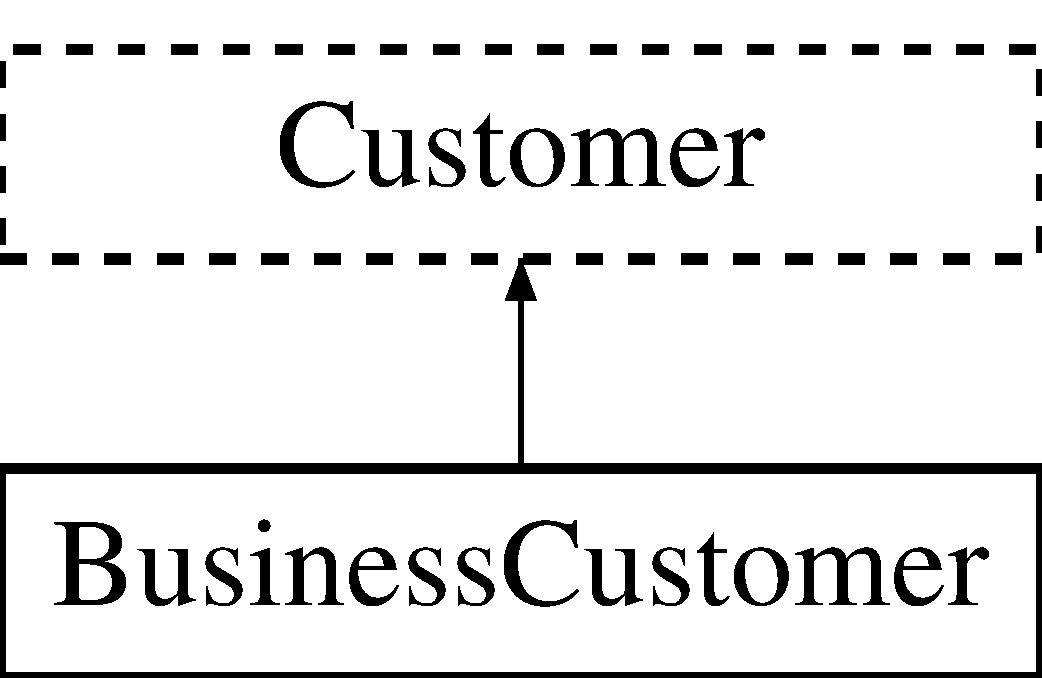
\includegraphics[height=2cm]{classBusinessCustomer}
\end{center}
\end{figure}
\subsection*{Public Member Functions}
\begin{CompactItemize}
\item 
\hyperlink{classBusinessCustomer_c8a0dcdb32d7a866c7383824889bfbae}{BusinessCustomer} (const string \&name=\char`\"{}UNKNOWN\char`\"{}, const string \&reg=\char`\"{}000000000\char`\"{})
\begin{CompactList}\small\item\em Create a business customer with a name, and registration number. \item\end{CompactList}\item 
virtual \hyperlink{classCustomer}{Customer} $\ast$ \hyperlink{classBusinessCustomer_6aaf68c4c9f64ed6cbb24855664d7244}{clone} () const 
\begin{CompactList}\small\item\em return a copy of yourself \item\end{CompactList}\item 
virtual istream \& \hyperlink{classBusinessCustomer_2c5cee8ad65d72e620a32f10e99b823d}{read} (istream \&is)  throw (input\_\-format\_\-error)
\begin{CompactList}\small\item\em Reads the information for a business customer from a stream. \item\end{CompactList}\item 
virtual ostream \& \hyperlink{classBusinessCustomer_2ea38f4b72488c8e9d7f7c38ed93b454}{write} (ostream \&os) const 
\begin{CompactList}\small\item\em Writes the information for a business customer to a stream. \item\end{CompactList}\end{CompactItemize}


\subsection{Constructor \& Destructor Documentation}
\hypertarget{classBusinessCustomer_c8a0dcdb32d7a866c7383824889bfbae}{
\index{BusinessCustomer@{BusinessCustomer}!BusinessCustomer@{BusinessCustomer}}
\index{BusinessCustomer@{BusinessCustomer}!BusinessCustomer@{BusinessCustomer}}
\subsubsection[BusinessCustomer]{\setlength{\rightskip}{0pt plus 5cm}BusinessCustomer::BusinessCustomer (const string \& {\em name} = {\tt \char`\"{}UNKNOWN\char`\"{}}, \/  const string \& {\em reg} = {\tt \char`\"{}000000000\char`\"{}})\hspace{0.3cm}{\tt  \mbox{[}inline\mbox{]}}}}
\label{classBusinessCustomer_c8a0dcdb32d7a866c7383824889bfbae}


\begin{Desc}
\item[Parameters:]
\begin{description}
\item[\mbox{$\leftarrow$} {\em name}]this business customer's name; defaults to {\bf UNKNOWN} \item[\mbox{$\leftarrow$} {\em reg}]this business customer's registration number; defaults to 000000000 \end{description}
\end{Desc}


\subsection{Member Function Documentation}
\hypertarget{classBusinessCustomer_6aaf68c4c9f64ed6cbb24855664d7244}{
\index{BusinessCustomer@{BusinessCustomer}!clone@{clone}}
\index{clone@{clone}!BusinessCustomer@{BusinessCustomer}}
\subsubsection[clone]{\setlength{\rightskip}{0pt plus 5cm}{\bf Customer} $\ast$ BusinessCustomer::clone () const\hspace{0.3cm}{\tt  \mbox{[}virtual\mbox{]}}}}
\label{classBusinessCustomer_6aaf68c4c9f64ed6cbb24855664d7244}


\begin{Desc}
\item[Returns:]a pointer to a copy of a \hyperlink{classBusinessCustomer}{BusinessCustomer} \end{Desc}


Implements \hyperlink{classCustomer_406fb74a887e5f0eb91aa49301534bb4}{Customer}.\hypertarget{classBusinessCustomer_2c5cee8ad65d72e620a32f10e99b823d}{
\index{BusinessCustomer@{BusinessCustomer}!read@{read}}
\index{read@{read}!BusinessCustomer@{BusinessCustomer}}
\subsubsection[read]{\setlength{\rightskip}{0pt plus 5cm}istream \& BusinessCustomer::read (istream \& {\em is})  throw (input\_\-format\_\-error)\hspace{0.3cm}{\tt  \mbox{[}virtual\mbox{]}}}}
\label{classBusinessCustomer_2c5cee8ad65d72e620a32f10e99b823d}


\begin{Desc}
\item[Parameters:]
\begin{description}
\item[\mbox{$\leftrightarrow$} {\em is}]the stream to read from and the updated stream \end{description}
\end{Desc}
\begin{Desc}
\item[Exceptions:]
\begin{description}
\item[{\em thrown}]if the account number is incorrectly written \end{description}
\end{Desc}
\begin{Desc}
\item[Returns:]the updated stream, so that it can be cascaded \end{Desc}


Implements \hyperlink{classCustomer_3327c4e5e7f3a9435f3b71372778386a}{Customer}.\hypertarget{classBusinessCustomer_2ea38f4b72488c8e9d7f7c38ed93b454}{
\index{BusinessCustomer@{BusinessCustomer}!write@{write}}
\index{write@{write}!BusinessCustomer@{BusinessCustomer}}
\subsubsection[write]{\setlength{\rightskip}{0pt plus 5cm}ostream \& BusinessCustomer::write (ostream \& {\em os}) const\hspace{0.3cm}{\tt  \mbox{[}virtual\mbox{]}}}}
\label{classBusinessCustomer_2ea38f4b72488c8e9d7f7c38ed93b454}


\begin{Desc}
\item[Parameters:]
\begin{description}
\item[\mbox{$\leftrightarrow$} {\em os}]the stream to write to and the updated stream \end{description}
\end{Desc}
\begin{Desc}
\item[Returns:]the updated stream, so that it can be cascaded \end{Desc}


Implements \hyperlink{classCustomer_a4ef104426d09a4817cb2d55e5e674d0}{Customer}.

The documentation for this class was generated from the following files:\begin{CompactItemize}
\item 
\hyperlink{businessCustomer_8h}{businessCustomer.h}\item 
\hyperlink{businessCustomer_8cc}{businessCustomer.cc}\end{CompactItemize}

\hypertarget{classChequingAccount}{
\section{ChequingAccount Class Reference}
\label{classChequingAccount}\index{ChequingAccount@{ChequingAccount}}
}
A simple abstract base class to represent a \hyperlink{classChequingAccount}{ChequingAccount}.  


{\tt \#include $<$chequingAccount.h$>$}

Inheritance diagram for ChequingAccount::\begin{figure}[H]
\begin{center}
\leavevmode
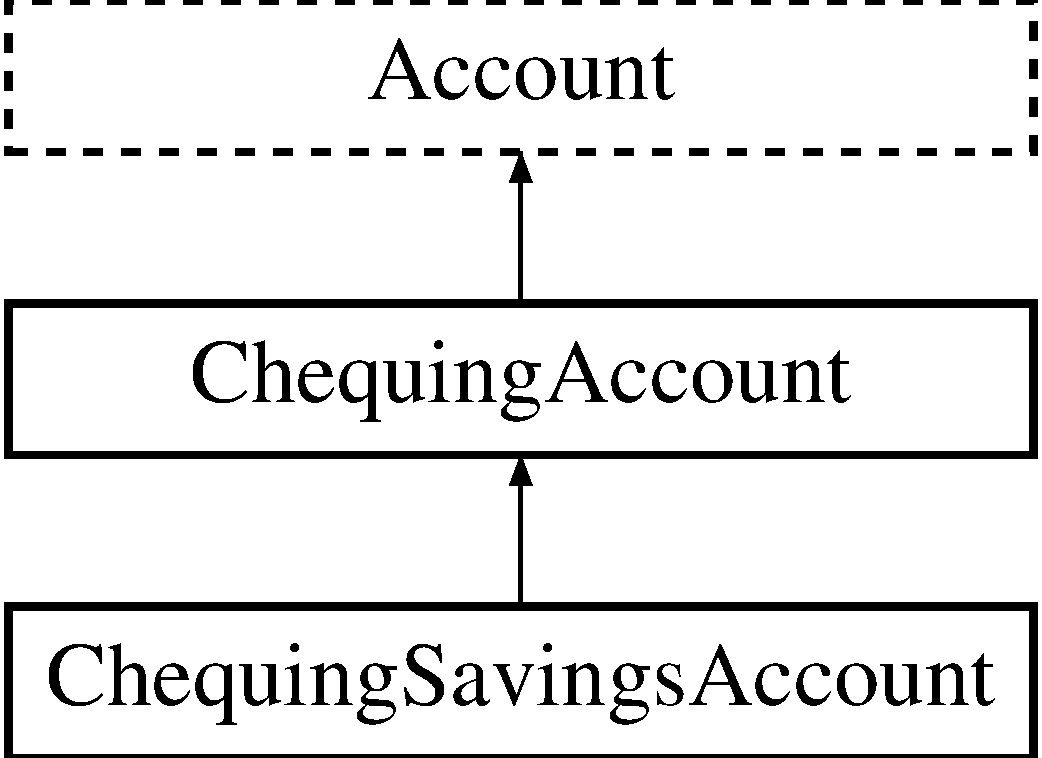
\includegraphics[height=3cm]{classChequingAccount}
\end{center}
\end{figure}
\subsection*{Public Member Functions}
\begin{CompactItemize}
\item 
\hyperlink{classChequingAccount_abe675fa503c8abfdee3913d35b52197}{ChequingAccount} (int numFree=0, int howMany=0, int fee=0)
\begin{CompactList}\small\item\em default constructor \item\end{CompactList}\item 
virtual istream \& \hyperlink{classChequingAccount_b0aaf92f019e79f95c39a0f6996acbf5}{read} (istream \&is)  throw (input\_\-format\_\-error)
\begin{CompactList}\small\item\em Reads all information for a chequing account, from a stream. \item\end{CompactList}\item 
virtual ostream \& \hyperlink{classChequingAccount_b85b405548099388a5d7866ed9065d33}{write} (ostream \&os) const 
\begin{CompactList}\small\item\em Writes all information for a chequing account, to a stream. \item\end{CompactList}\item 
virtual void \hyperlink{classChequingAccount_14b54359ca8a5260b7decf0aa9bb04d2}{withdraw} (int amount)  throw (insufficient\_\-funds)
\begin{CompactList}\small\item\em Withdraws {\em amount\/} from this account. \item\end{CompactList}\item 
virtual void \hyperlink{classChequingAccount_03a0e06869ce9180c4e7ef2fdb39e616}{updateMonthEnd} ()
\begin{CompactList}\small\item\em Performs updates to the account at the end of the month. \item\end{CompactList}\end{CompactItemize}
\subsection*{Protected Member Functions}
\begin{CompactItemize}
\item 
virtual istream \& \hyperlink{classChequingAccount_09de2d9912d5f817b651659404549111}{readExtra} (istream \&is)
\begin{CompactList}\small\item\em Reads the information,specific to a chequing account, from a stream. \item\end{CompactList}\item 
virtual ostream \& \hyperlink{classChequingAccount_5f2831100ca8357b9d74a1402477f3f6}{writeExtra} (ostream \&os) const 
\begin{CompactList}\small\item\em Writes the information, specific to a chequing account, to a stream. \item\end{CompactList}\end{CompactItemize}


\subsection{Constructor \& Destructor Documentation}
\hypertarget{classChequingAccount_abe675fa503c8abfdee3913d35b52197}{
\index{ChequingAccount@{ChequingAccount}!ChequingAccount@{ChequingAccount}}
\index{ChequingAccount@{ChequingAccount}!ChequingAccount@{ChequingAccount}}
\subsubsection[ChequingAccount]{\setlength{\rightskip}{0pt plus 5cm}ChequingAccount::ChequingAccount (int {\em numFree} = {\tt 0}, \/  int {\em howMany} = {\tt 0}, \/  int {\em fee} = {\tt 0})\hspace{0.3cm}{\tt  \mbox{[}inline\mbox{]}}}}
\label{classChequingAccount_abe675fa503c8abfdee3913d35b52197}


\begin{Desc}
\item[Parameters:]
\begin{description}
\item[{\em numFree}]imports the number of free withdrawals allowed \item[{\em howMany}]imports the number of withdrawals made \item[{\em fee}]imports the fee to be charged for a withdrawal \end{description}
\end{Desc}


\subsection{Member Function Documentation}
\hypertarget{classChequingAccount_b0aaf92f019e79f95c39a0f6996acbf5}{
\index{ChequingAccount@{ChequingAccount}!read@{read}}
\index{read@{read}!ChequingAccount@{ChequingAccount}}
\subsubsection[read]{\setlength{\rightskip}{0pt plus 5cm}istream \& ChequingAccount::read (istream \& {\em is})  throw (input\_\-format\_\-error)\hspace{0.3cm}{\tt  \mbox{[}virtual\mbox{]}}}}
\label{classChequingAccount_b0aaf92f019e79f95c39a0f6996acbf5}


\begin{Desc}
\item[Parameters:]
\begin{description}
\item[\mbox{$\leftrightarrow$} {\em is}]the stream to read from and the updated stream \end{description}
\end{Desc}
\begin{Desc}
\item[Exceptions:]
\begin{description}
\item[{\em thrown}]from account::read() \end{description}
\end{Desc}
\begin{Desc}
\item[Returns:]the updated stream, so that it can be cascaded \end{Desc}


Reimplemented from \hyperlink{classAccount_1ef84736fe231b64547ba0b7824ac7c6}{Account}.

Reimplemented in \hyperlink{classChequingSavingsAccount_c0de0e2d3ac55227f31a4715ae257646}{ChequingSavingsAccount}.

References Account::read().\hypertarget{classChequingAccount_b85b405548099388a5d7866ed9065d33}{
\index{ChequingAccount@{ChequingAccount}!write@{write}}
\index{write@{write}!ChequingAccount@{ChequingAccount}}
\subsubsection[write]{\setlength{\rightskip}{0pt plus 5cm}ostream \& ChequingAccount::write (ostream \& {\em os}) const\hspace{0.3cm}{\tt  \mbox{[}virtual\mbox{]}}}}
\label{classChequingAccount_b85b405548099388a5d7866ed9065d33}


\begin{Desc}
\item[Parameters:]
\begin{description}
\item[\mbox{$\leftrightarrow$} {\em os}]the stream to write to and the updated stream \end{description}
\end{Desc}
\begin{Desc}
\item[Returns:]the updated stream, so that it can be cascaded \end{Desc}


Reimplemented from \hyperlink{classAccount_65f80b996aecc07bcb5ddd31fcb0b063}{Account}.

Reimplemented in \hyperlink{classChequingSavingsAccount_61888979bbaf273b2c20f92d2f41f226}{ChequingSavingsAccount}.

References Account::write(), and writeExtra().\hypertarget{classChequingAccount_14b54359ca8a5260b7decf0aa9bb04d2}{
\index{ChequingAccount@{ChequingAccount}!withdraw@{withdraw}}
\index{withdraw@{withdraw}!ChequingAccount@{ChequingAccount}}
\subsubsection[withdraw]{\setlength{\rightskip}{0pt plus 5cm}void ChequingAccount::withdraw (int {\em amount})  throw (insufficient\_\-funds)\hspace{0.3cm}{\tt  \mbox{[}virtual\mbox{]}}}}
\label{classChequingAccount_14b54359ca8a5260b7decf0aa9bb04d2}


\begin{Desc}
\item[Parameters:]
\begin{description}
\item[\mbox{$\leftarrow$} {\em amount}]imports the amount to be withdrawn \end{description}
\end{Desc}
\begin{Desc}
\item[Exceptions:]
\begin{description}
\item[{\em thrown}]if the balance is less than the desired amount \end{description}
\end{Desc}
\begin{Desc}
\item[Postcondition:]the balance has been increased by amount plus any service charges \end{Desc}


Reimplemented from \hyperlink{classAccount_d239379460e2b8975bc8472514768850}{Account}.

References Account::balance.\hypertarget{classChequingAccount_03a0e06869ce9180c4e7ef2fdb39e616}{
\index{ChequingAccount@{ChequingAccount}!updateMonthEnd@{updateMonthEnd}}
\index{updateMonthEnd@{updateMonthEnd}!ChequingAccount@{ChequingAccount}}
\subsubsection[updateMonthEnd]{\setlength{\rightskip}{0pt plus 5cm}void ChequingAccount::updateMonthEnd ()\hspace{0.3cm}{\tt  \mbox{[}virtual\mbox{]}}}}
\label{classChequingAccount_03a0e06869ce9180c4e7ef2fdb39e616}


\begin{Desc}
\item[Postcondition:]the number of withdrawals has been set to 0 \end{Desc}


Implements \hyperlink{classAccount_3823d2d885625b78f83088946c257697}{Account}.

Reimplemented in \hyperlink{classChequingSavingsAccount_0bbd0c3b03b968fc2f80eb2a4fffa3f2}{ChequingSavingsAccount}.

Referenced by ChequingSavingsAccount::updateMonthEnd().\hypertarget{classChequingAccount_09de2d9912d5f817b651659404549111}{
\index{ChequingAccount@{ChequingAccount}!readExtra@{readExtra}}
\index{readExtra@{readExtra}!ChequingAccount@{ChequingAccount}}
\subsubsection[readExtra]{\setlength{\rightskip}{0pt plus 5cm}istream \& ChequingAccount::readExtra (istream \& {\em is})\hspace{0.3cm}{\tt  \mbox{[}protected, virtual\mbox{]}}}}
\label{classChequingAccount_09de2d9912d5f817b651659404549111}


\begin{Desc}
\item[Parameters:]
\begin{description}
\item[\mbox{$\leftrightarrow$} {\em is}]the stream to read from and the updated stream \end{description}
\end{Desc}
\begin{Desc}
\item[Returns:]the updated stream, so that it can be cascaded \end{Desc}


Referenced by ChequingSavingsAccount::read().\hypertarget{classChequingAccount_5f2831100ca8357b9d74a1402477f3f6}{
\index{ChequingAccount@{ChequingAccount}!writeExtra@{writeExtra}}
\index{writeExtra@{writeExtra}!ChequingAccount@{ChequingAccount}}
\subsubsection[writeExtra]{\setlength{\rightskip}{0pt plus 5cm}ostream \& ChequingAccount::writeExtra (ostream \& {\em os}) const\hspace{0.3cm}{\tt  \mbox{[}protected, virtual\mbox{]}}}}
\label{classChequingAccount_5f2831100ca8357b9d74a1402477f3f6}


\begin{Desc}
\item[Parameters:]
\begin{description}
\item[\mbox{$\leftrightarrow$} {\em os}]the stream to write to and the updated stream \end{description}
\end{Desc}
\begin{Desc}
\item[Returns:]the updated stream, so that it can be cascaded \end{Desc}


Referenced by ChequingSavingsAccount::write(), and write().

The documentation for this class was generated from the following files:\begin{CompactItemize}
\item 
\hyperlink{chequingAccount_8h}{chequingAccount.h}\item 
\hyperlink{chequingAccount_8cc}{chequingAccount.cc}\end{CompactItemize}

\hypertarget{classChequingSavingsAccount}{
\section{ChequingSavingsAccount Class Reference}
\label{classChequingSavingsAccount}\index{ChequingSavingsAccount@{ChequingSavingsAccount}}
}
A concrete derived class to represent a \hyperlink{classChequingSavingsAccount}{ChequingSavingsAccount}.  


{\tt \#include $<$chequingSavingsAccount.h$>$}

Inheritance diagram for ChequingSavingsAccount::\begin{figure}[H]
\begin{center}
\leavevmode
\includegraphics[height=3cm]{classChequingSavingsAccount}
\end{center}
\end{figure}
\subsection*{Public Member Functions}
\begin{CompactItemize}
\item 
\hyperlink{classChequingSavingsAccount_97bbf69acfaedb5e8442528b24f10480}{ChequingSavingsAccount} (double rate=0.0, int numFree=0, int howMany=0, int fee=0)
\begin{CompactList}\small\item\em default constructor \item\end{CompactList}\item 
virtual istream \& \hyperlink{classChequingSavingsAccount_c0de0e2d3ac55227f31a4715ae257646}{read} (istream \&is)  throw (input\_\-format\_\-error)
\begin{CompactList}\small\item\em Reads all information for a chequing savings account, from a stream. \item\end{CompactList}\item 
virtual ostream \& \hyperlink{classChequingSavingsAccount_61888979bbaf273b2c20f92d2f41f226}{write} (ostream \&os) const 
\begin{CompactList}\small\item\em Writes all information for a chequing savings account, to a stream. \item\end{CompactList}\item 
virtual void \hyperlink{classChequingSavingsAccount_0bbd0c3b03b968fc2f80eb2a4fffa3f2}{updateMonthEnd} ()
\begin{CompactList}\small\item\em Performs updates to the account at the end of the month. \item\end{CompactList}\end{CompactItemize}


\subsection{Constructor \& Destructor Documentation}
\hypertarget{classChequingSavingsAccount_97bbf69acfaedb5e8442528b24f10480}{
\index{ChequingSavingsAccount@{ChequingSavingsAccount}!ChequingSavingsAccount@{ChequingSavingsAccount}}
\index{ChequingSavingsAccount@{ChequingSavingsAccount}!ChequingSavingsAccount@{ChequingSavingsAccount}}
\subsubsection[ChequingSavingsAccount]{\setlength{\rightskip}{0pt plus 5cm}ChequingSavingsAccount::ChequingSavingsAccount (double {\em rate} = {\tt 0.0}, \/  int {\em numFree} = {\tt 0}, \/  int {\em howMany} = {\tt 0}, \/  int {\em fee} = {\tt 0})\hspace{0.3cm}{\tt  \mbox{[}inline\mbox{]}}}}
\label{classChequingSavingsAccount_97bbf69acfaedb5e8442528b24f10480}


\begin{Desc}
\item[Parameters:]
\begin{description}
\item[{\em rate}]imports the monthly interest rate as a percentage \item[{\em numFree}]imports the number of free withdrawals allowed \item[{\em howMany}]imports the number of withdrawals made \item[{\em fee}]imports the fee to be charged for a withdrawal \end{description}
\end{Desc}


\subsection{Member Function Documentation}
\hypertarget{classChequingSavingsAccount_c0de0e2d3ac55227f31a4715ae257646}{
\index{ChequingSavingsAccount@{ChequingSavingsAccount}!read@{read}}
\index{read@{read}!ChequingSavingsAccount@{ChequingSavingsAccount}}
\subsubsection[read]{\setlength{\rightskip}{0pt plus 5cm}istream \& ChequingSavingsAccount::read (istream \& {\em is})  throw (input\_\-format\_\-error)\hspace{0.3cm}{\tt  \mbox{[}virtual\mbox{]}}}}
\label{classChequingSavingsAccount_c0de0e2d3ac55227f31a4715ae257646}


\begin{Desc}
\item[Parameters:]
\begin{description}
\item[\mbox{$\leftrightarrow$} {\em is}]the stream to read from and the updated stream \end{description}
\end{Desc}
\begin{Desc}
\item[Exceptions:]
\begin{description}
\item[{\em thrown}]by account::read() if incorrect \end{description}
\end{Desc}
\begin{Desc}
\item[Returns:]the updated stream, so that it can be cascaded \end{Desc}


Reimplemented from \hyperlink{classChequingAccount_b0aaf92f019e79f95c39a0f6996acbf5}{ChequingAccount}.

References Account::read(), ChequingAccount::readExtra(), and SavingsAccount::readExtra().\hypertarget{classChequingSavingsAccount_61888979bbaf273b2c20f92d2f41f226}{
\index{ChequingSavingsAccount@{ChequingSavingsAccount}!write@{write}}
\index{write@{write}!ChequingSavingsAccount@{ChequingSavingsAccount}}
\subsubsection[write]{\setlength{\rightskip}{0pt plus 5cm}ostream \& ChequingSavingsAccount::write (ostream \& {\em os}) const\hspace{0.3cm}{\tt  \mbox{[}virtual\mbox{]}}}}
\label{classChequingSavingsAccount_61888979bbaf273b2c20f92d2f41f226}


\begin{Desc}
\item[Parameters:]
\begin{description}
\item[\mbox{$\leftrightarrow$} {\em os}]the stream to write to and the updated stream \end{description}
\end{Desc}
\begin{Desc}
\item[Returns:]the updated stream, so that it can be cascaded \end{Desc}


Reimplemented from \hyperlink{classChequingAccount_b85b405548099388a5d7866ed9065d33}{ChequingAccount}.

References Account::write(), ChequingAccount::writeExtra(), and SavingsAccount::writeExtra().\hypertarget{classChequingSavingsAccount_0bbd0c3b03b968fc2f80eb2a4fffa3f2}{
\index{ChequingSavingsAccount@{ChequingSavingsAccount}!updateMonthEnd@{updateMonthEnd}}
\index{updateMonthEnd@{updateMonthEnd}!ChequingSavingsAccount@{ChequingSavingsAccount}}
\subsubsection[updateMonthEnd]{\setlength{\rightskip}{0pt plus 5cm}void ChequingSavingsAccount::updateMonthEnd ()\hspace{0.3cm}{\tt  \mbox{[}virtual\mbox{]}}}}
\label{classChequingSavingsAccount_0bbd0c3b03b968fc2f80eb2a4fffa3f2}


\begin{Desc}
\item[Postcondition:]Interest earned has been added to the balance 

The number of withdrawals is reset to 0 \end{Desc}


Reimplemented from \hyperlink{classChequingAccount_03a0e06869ce9180c4e7ef2fdb39e616}{ChequingAccount}.

References ChequingAccount::updateMonthEnd(), and SavingsAccount::updateMonthEnd().

The documentation for this class was generated from the following files:\begin{CompactItemize}
\item 
\hyperlink{chequingSavingsAccount_8h}{chequingSavingsAccount.h}\item 
\hyperlink{chequingSavingsAccount_8cc}{chequingSavingsAccount.cc}\end{CompactItemize}

\hypertarget{classCustomer}{
\section{Customer Class Reference}
\label{classCustomer}\index{Customer@{Customer}}
}
A simple abstract base class to represent a \hyperlink{classCustomer}{Customer}.  


{\tt \#include $<$customer.h$>$}

Inheritance diagram for Customer::\begin{figure}[H]
\begin{center}
\leavevmode
\includegraphics[height=2cm]{classCustomer}
\end{center}
\end{figure}
\subsection*{Public Member Functions}
\begin{CompactItemize}
\item 
virtual \hyperlink{classCustomer_7784915654b180d09696edded3db913d}{$\sim$Customer} ()
\begin{CompactList}\small\item\em Virtual destructor. \item\end{CompactList}\item 
virtual \hyperlink{classCustomer}{Customer} $\ast$ \hyperlink{classCustomer_406fb74a887e5f0eb91aa49301534bb4}{clone} () const =0
\begin{CompactList}\small\item\em return a copy of yourself \item\end{CompactList}\item 
virtual istream \& \hyperlink{classCustomer_3327c4e5e7f3a9435f3b71372778386a}{read} (istream \&is)=0
\begin{CompactList}\small\item\em Reads the information for a \hyperlink{classCustomer}{Customer} from a stream. \item\end{CompactList}\item 
virtual ostream \& \hyperlink{classCustomer_a4ef104426d09a4817cb2d55e5e674d0}{write} (ostream \&os) const =0
\begin{CompactList}\small\item\em Writes the information for a \hyperlink{classCustomer}{Customer} to a stream. \item\end{CompactList}\end{CompactItemize}


\subsection{Constructor \& Destructor Documentation}
\hypertarget{classCustomer_7784915654b180d09696edded3db913d}{
\index{Customer@{Customer}!$\sim$Customer@{$\sim$Customer}}
\index{$\sim$Customer@{$\sim$Customer}!Customer@{Customer}}
\subsubsection[$\sim$Customer]{\setlength{\rightskip}{0pt plus 5cm}virtual Customer::$\sim$Customer ()\hspace{0.3cm}{\tt  \mbox{[}inline, virtual\mbox{]}}}}
\label{classCustomer_7784915654b180d09696edded3db913d}


This function does nothing. It is provided so that sub class objects are correctly destroyed 

\subsection{Member Function Documentation}
\hypertarget{classCustomer_406fb74a887e5f0eb91aa49301534bb4}{
\index{Customer@{Customer}!clone@{clone}}
\index{clone@{clone}!Customer@{Customer}}
\subsubsection[clone]{\setlength{\rightskip}{0pt plus 5cm}virtual {\bf Customer}$\ast$ Customer::clone () const\hspace{0.3cm}{\tt  \mbox{[}pure virtual\mbox{]}}}}
\label{classCustomer_406fb74a887e5f0eb91aa49301534bb4}


\begin{Desc}
\item[Returns:]a pointer to a copy of the current customer \end{Desc}


Implemented in \hyperlink{classBusinessCustomer_6aaf68c4c9f64ed6cbb24855664d7244}{BusinessCustomer}, and \hyperlink{classPersonalCustomer_a1e9e9e14356c0ff7a3d97c999e44388}{PersonalCustomer}.\hypertarget{classCustomer_3327c4e5e7f3a9435f3b71372778386a}{
\index{Customer@{Customer}!read@{read}}
\index{read@{read}!Customer@{Customer}}
\subsubsection[read]{\setlength{\rightskip}{0pt plus 5cm}virtual istream\& Customer::read (istream \& {\em is})\hspace{0.3cm}{\tt  \mbox{[}pure virtual\mbox{]}}}}
\label{classCustomer_3327c4e5e7f3a9435f3b71372778386a}


\begin{Desc}
\item[Parameters:]
\begin{description}
\item[\mbox{$\leftrightarrow$} {\em is}]the stream to read from and the updated stream \end{description}
\end{Desc}
\begin{Desc}
\item[Returns:]the updated stream, so that it can be cascaded \end{Desc}


Implemented in \hyperlink{classBusinessCustomer_2c5cee8ad65d72e620a32f10e99b823d}{BusinessCustomer}, and \hyperlink{classPersonalCustomer_81861fd3353273de8c4da5f273ecfd26}{PersonalCustomer}.

Referenced by operator$>$$>$().\hypertarget{classCustomer_a4ef104426d09a4817cb2d55e5e674d0}{
\index{Customer@{Customer}!write@{write}}
\index{write@{write}!Customer@{Customer}}
\subsubsection[write]{\setlength{\rightskip}{0pt plus 5cm}virtual ostream\& Customer::write (ostream \& {\em os}) const\hspace{0.3cm}{\tt  \mbox{[}pure virtual\mbox{]}}}}
\label{classCustomer_a4ef104426d09a4817cb2d55e5e674d0}


\begin{Desc}
\item[Parameters:]
\begin{description}
\item[\mbox{$\leftrightarrow$} {\em os}]the stream to write to and the updated stream \end{description}
\end{Desc}
\begin{Desc}
\item[Returns:]the updated stream, so that it can be cascaded \end{Desc}


Implemented in \hyperlink{classBusinessCustomer_2ea38f4b72488c8e9d7f7c38ed93b454}{BusinessCustomer}, and \hyperlink{classPersonalCustomer_123975841172a6933c0358907d29f495}{PersonalCustomer}.

Referenced by operator$<$$<$().

The documentation for this class was generated from the following file:\begin{CompactItemize}
\item 
\hyperlink{customer_8h}{customer.h}\end{CompactItemize}

\hypertarget{classPersonalCustomer}{
\section{PersonalCustomer Class Reference}
\label{classPersonalCustomer}\index{PersonalCustomer@{PersonalCustomer}}
}
A simple class to represent a \hyperlink{classPersonalCustomer}{PersonalCustomer} who IS A \hyperlink{classCustomer}{Customer}.  


{\tt \#include $<$personalCustomer.h$>$}

Inheritance diagram for PersonalCustomer::\begin{figure}[H]
\begin{center}
\leavevmode
\includegraphics[height=2cm]{classPersonalCustomer}
\end{center}
\end{figure}
\subsection*{Public Member Functions}
\begin{CompactItemize}
\item 
\hyperlink{classPersonalCustomer_a85bdbac31d8424ff81a44d803fbec53}{PersonalCustomer} (const string \&name=\char`\"{}UNKNOWN\char`\"{}, const string \&sin=\char`\"{}000000000\char`\"{})
\begin{CompactList}\small\item\em Create a personal customer with a name, and SIN. \item\end{CompactList}\item 
virtual \hyperlink{classCustomer}{Customer} $\ast$ \hyperlink{classPersonalCustomer_a1e9e9e14356c0ff7a3d97c999e44388}{clone} () const 
\begin{CompactList}\small\item\em return a copy of yourself \item\end{CompactList}\item 
virtual istream \& \hyperlink{classPersonalCustomer_81861fd3353273de8c4da5f273ecfd26}{read} (istream \&is)  throw (input\_\-format\_\-error)
\begin{CompactList}\small\item\em Reads the information for a personal customer from a stream. \item\end{CompactList}\item 
virtual ostream \& \hyperlink{classPersonalCustomer_123975841172a6933c0358907d29f495}{write} (ostream \&os) const 
\begin{CompactList}\small\item\em Writes the information for a personal customer to a stream. \item\end{CompactList}\end{CompactItemize}


\subsection{Constructor \& Destructor Documentation}
\hypertarget{classPersonalCustomer_a85bdbac31d8424ff81a44d803fbec53}{
\index{PersonalCustomer@{PersonalCustomer}!PersonalCustomer@{PersonalCustomer}}
\index{PersonalCustomer@{PersonalCustomer}!PersonalCustomer@{PersonalCustomer}}
\subsubsection[PersonalCustomer]{\setlength{\rightskip}{0pt plus 5cm}PersonalCustomer::PersonalCustomer (const string \& {\em name} = {\tt \char`\"{}UNKNOWN\char`\"{}}, \/  const string \& {\em sin} = {\tt \char`\"{}000000000\char`\"{}})\hspace{0.3cm}{\tt  \mbox{[}inline\mbox{]}}}}
\label{classPersonalCustomer_a85bdbac31d8424ff81a44d803fbec53}


\begin{Desc}
\item[Parameters:]
\begin{description}
\item[\mbox{$\leftarrow$} {\em name}]this personal customer's name; default {\bf UNKNOWN} \item[\mbox{$\leftarrow$} {\em sin}]this personal customer's SIN; defaults to 000000000 \end{description}
\end{Desc}


\subsection{Member Function Documentation}
\hypertarget{classPersonalCustomer_a1e9e9e14356c0ff7a3d97c999e44388}{
\index{PersonalCustomer@{PersonalCustomer}!clone@{clone}}
\index{clone@{clone}!PersonalCustomer@{PersonalCustomer}}
\subsubsection[clone]{\setlength{\rightskip}{0pt plus 5cm}{\bf Customer} $\ast$ PersonalCustomer::clone () const\hspace{0.3cm}{\tt  \mbox{[}virtual\mbox{]}}}}
\label{classPersonalCustomer_a1e9e9e14356c0ff7a3d97c999e44388}


\begin{Desc}
\item[Returns:]a pointer to a copy of a \hyperlink{classPersonalCustomer}{PersonalCustomer} \end{Desc}


Implements \hyperlink{classCustomer_406fb74a887e5f0eb91aa49301534bb4}{Customer}.\hypertarget{classPersonalCustomer_81861fd3353273de8c4da5f273ecfd26}{
\index{PersonalCustomer@{PersonalCustomer}!read@{read}}
\index{read@{read}!PersonalCustomer@{PersonalCustomer}}
\subsubsection[read]{\setlength{\rightskip}{0pt plus 5cm}istream \& PersonalCustomer::read (istream \& {\em is})  throw (input\_\-format\_\-error)\hspace{0.3cm}{\tt  \mbox{[}virtual\mbox{]}}}}
\label{classPersonalCustomer_81861fd3353273de8c4da5f273ecfd26}


\begin{Desc}
\item[Parameters:]
\begin{description}
\item[\mbox{$\leftrightarrow$} {\em is}]the stream to read from and the updated stream \end{description}
\end{Desc}
\begin{Desc}
\item[Exceptions:]
\begin{description}
\item[{\em thrown}]if the SIN is of incorrect length or if it contains alphabetic characters \end{description}
\end{Desc}
\begin{Desc}
\item[Returns:]the updated stream, so that it can be cascaded \end{Desc}


Implements \hyperlink{classCustomer_3327c4e5e7f3a9435f3b71372778386a}{Customer}.\hypertarget{classPersonalCustomer_123975841172a6933c0358907d29f495}{
\index{PersonalCustomer@{PersonalCustomer}!write@{write}}
\index{write@{write}!PersonalCustomer@{PersonalCustomer}}
\subsubsection[write]{\setlength{\rightskip}{0pt plus 5cm}ostream \& PersonalCustomer::write (ostream \& {\em os}) const\hspace{0.3cm}{\tt  \mbox{[}virtual\mbox{]}}}}
\label{classPersonalCustomer_123975841172a6933c0358907d29f495}


\begin{Desc}
\item[Parameters:]
\begin{description}
\item[\mbox{$\leftrightarrow$} {\em os}]the stream to write to and the updated stream \end{description}
\end{Desc}
\begin{Desc}
\item[Returns:]the updated stream, so that it can be cascaded \end{Desc}


Implements \hyperlink{classCustomer_a4ef104426d09a4817cb2d55e5e674d0}{Customer}.

The documentation for this class was generated from the following files:\begin{CompactItemize}
\item 
\hyperlink{personalCustomer_8h}{personalCustomer.h}\item 
\hyperlink{personalCustomer_8cc}{personalCustomer.cc}\end{CompactItemize}

\hypertarget{classSavingsAccount}{
\section{SavingsAccount Class Reference}
\label{classSavingsAccount}\index{SavingsAccount@{SavingsAccount}}
}
A simple abstract base class to represent a \hyperlink{classSavingsAccount}{SavingsAccount}.  


{\tt \#include $<$savingsAccount.h$>$}

Inheritance diagram for SavingsAccount::\begin{figure}[H]
\begin{center}
\leavevmode
\includegraphics[height=3cm]{classSavingsAccount}
\end{center}
\end{figure}
\subsection*{Public Member Functions}
\begin{CompactItemize}
\item 
\hyperlink{classSavingsAccount_b7517ac4a985dc029f2587109c984482}{SavingsAccount} (double rate=0.0)
\begin{CompactList}\small\item\em default constructor \item\end{CompactList}\item 
virtual istream \& \hyperlink{classSavingsAccount_a738133ea37093f4e0ae9d3a6dc14674}{read} (istream \&is)  throw (input\_\-format\_\-error)
\begin{CompactList}\small\item\em Reads all information for a savings account, from a stream. \item\end{CompactList}\item 
virtual ostream \& \hyperlink{classSavingsAccount_7010b1663ff729cb05a3594c7bc8ae99}{write} (ostream \&os) const 
\begin{CompactList}\small\item\em Writes all information for a savings account, to a stream. \item\end{CompactList}\item 
virtual void \hyperlink{classSavingsAccount_fedffc6bb917570025ac1e30db9e4f76}{updateMonthEnd} ()
\begin{CompactList}\small\item\em Performs updates to the account at the end of the month. \item\end{CompactList}\end{CompactItemize}
\subsection*{Protected Member Functions}
\begin{CompactItemize}
\item 
virtual istream \& \hyperlink{classSavingsAccount_3afc54ec8471fb44d804750ebe63e1c9}{readExtra} (istream \&is)
\begin{CompactList}\small\item\em Reads the information,specific to savings account, from a stream. \item\end{CompactList}\item 
virtual ostream \& \hyperlink{classSavingsAccount_6a2fce79d1bde2580c291847ec1cf989}{writeExtra} (ostream \&os) const 
\begin{CompactList}\small\item\em Writes the information, specific to a savings account, to a stream. \item\end{CompactList}\end{CompactItemize}
\subsection*{Protected Attributes}
\begin{CompactItemize}
\item 
\hypertarget{classSavingsAccount_de464fb646c70277052a60e9d098f511}{
double \hyperlink{classSavingsAccount_de464fb646c70277052a60e9d098f511}{interestRate}}
\label{classSavingsAccount_de464fb646c70277052a60e9d098f511}

\begin{CompactList}\small\item\em The monthly interest rate as a percentage. \item\end{CompactList}\end{CompactItemize}


\subsection{Constructor \& Destructor Documentation}
\hypertarget{classSavingsAccount_b7517ac4a985dc029f2587109c984482}{
\index{SavingsAccount@{SavingsAccount}!SavingsAccount@{SavingsAccount}}
\index{SavingsAccount@{SavingsAccount}!SavingsAccount@{SavingsAccount}}
\subsubsection[SavingsAccount]{\setlength{\rightskip}{0pt plus 5cm}SavingsAccount::SavingsAccount (double {\em rate} = {\tt 0.0})\hspace{0.3cm}{\tt  \mbox{[}inline\mbox{]}}}}
\label{classSavingsAccount_b7517ac4a985dc029f2587109c984482}


Create a savings account with the specified interest rate

\begin{Desc}
\item[Parameters:]
\begin{description}
\item[{\em rate}]imports the monthly interest rate as a percentage \end{description}
\end{Desc}


\subsection{Member Function Documentation}
\hypertarget{classSavingsAccount_a738133ea37093f4e0ae9d3a6dc14674}{
\index{SavingsAccount@{SavingsAccount}!read@{read}}
\index{read@{read}!SavingsAccount@{SavingsAccount}}
\subsubsection[read]{\setlength{\rightskip}{0pt plus 5cm}istream \& SavingsAccount::read (istream \& {\em is})  throw (input\_\-format\_\-error)\hspace{0.3cm}{\tt  \mbox{[}virtual\mbox{]}}}}
\label{classSavingsAccount_a738133ea37093f4e0ae9d3a6dc14674}


\begin{Desc}
\item[Parameters:]
\begin{description}
\item[\mbox{$\leftrightarrow$} {\em is}]the stream to read from and the updated stream \end{description}
\end{Desc}
\begin{Desc}
\item[Exceptions:]
\begin{description}
\item[{\em thrown}]when the input cannot be correctly interpreted \end{description}
\end{Desc}
\begin{Desc}
\item[Returns:]the updated stream, so that it can be cascaded \end{Desc}


Reimplemented from \hyperlink{classAccount_1ef84736fe231b64547ba0b7824ac7c6}{Account}.

Reimplemented in \hyperlink{classChequingSavingsAccount_c0de0e2d3ac55227f31a4715ae257646}{ChequingSavingsAccount}.

References Account::read().\hypertarget{classSavingsAccount_7010b1663ff729cb05a3594c7bc8ae99}{
\index{SavingsAccount@{SavingsAccount}!write@{write}}
\index{write@{write}!SavingsAccount@{SavingsAccount}}
\subsubsection[write]{\setlength{\rightskip}{0pt plus 5cm}ostream \& SavingsAccount::write (ostream \& {\em os}) const\hspace{0.3cm}{\tt  \mbox{[}virtual\mbox{]}}}}
\label{classSavingsAccount_7010b1663ff729cb05a3594c7bc8ae99}


\begin{Desc}
\item[Parameters:]
\begin{description}
\item[\mbox{$\leftrightarrow$} {\em os}]the stream to write to and the updated stream \end{description}
\end{Desc}
\begin{Desc}
\item[Returns:]the updated stream, so that it can be cascaded \end{Desc}


Reimplemented from \hyperlink{classAccount_65f80b996aecc07bcb5ddd31fcb0b063}{Account}.

Reimplemented in \hyperlink{classChequingSavingsAccount_61888979bbaf273b2c20f92d2f41f226}{ChequingSavingsAccount}.

References Account::write(), and writeExtra().\hypertarget{classSavingsAccount_fedffc6bb917570025ac1e30db9e4f76}{
\index{SavingsAccount@{SavingsAccount}!updateMonthEnd@{updateMonthEnd}}
\index{updateMonthEnd@{updateMonthEnd}!SavingsAccount@{SavingsAccount}}
\subsubsection[updateMonthEnd]{\setlength{\rightskip}{0pt plus 5cm}void SavingsAccount::updateMonthEnd ()\hspace{0.3cm}{\tt  \mbox{[}virtual\mbox{]}}}}
\label{classSavingsAccount_fedffc6bb917570025ac1e30db9e4f76}


This function will calculate and add the interest earned to the balance at the end of the month.

\begin{Desc}
\item[Postcondition:]the balance is increased by the amount of interest earned \end{Desc}


Implements \hyperlink{classAccount_3823d2d885625b78f83088946c257697}{Account}.

Reimplemented in \hyperlink{classChequingSavingsAccount_0bbd0c3b03b968fc2f80eb2a4fffa3f2}{ChequingSavingsAccount}.

References Account::balance, and interestRate.

Referenced by ChequingSavingsAccount::updateMonthEnd().\hypertarget{classSavingsAccount_3afc54ec8471fb44d804750ebe63e1c9}{
\index{SavingsAccount@{SavingsAccount}!readExtra@{readExtra}}
\index{readExtra@{readExtra}!SavingsAccount@{SavingsAccount}}
\subsubsection[readExtra]{\setlength{\rightskip}{0pt plus 5cm}istream \& SavingsAccount::readExtra (istream \& {\em is})\hspace{0.3cm}{\tt  \mbox{[}protected, virtual\mbox{]}}}}
\label{classSavingsAccount_3afc54ec8471fb44d804750ebe63e1c9}


\begin{Desc}
\item[Parameters:]
\begin{description}
\item[\mbox{$\leftrightarrow$} {\em is}]the stream to read from and the updated stream \end{description}
\end{Desc}
\begin{Desc}
\item[Returns:]the updated stream, so that it can be cascaded \end{Desc}


References interestRate.

Referenced by ChequingSavingsAccount::read().\hypertarget{classSavingsAccount_6a2fce79d1bde2580c291847ec1cf989}{
\index{SavingsAccount@{SavingsAccount}!writeExtra@{writeExtra}}
\index{writeExtra@{writeExtra}!SavingsAccount@{SavingsAccount}}
\subsubsection[writeExtra]{\setlength{\rightskip}{0pt plus 5cm}ostream \& SavingsAccount::writeExtra (ostream \& {\em os}) const\hspace{0.3cm}{\tt  \mbox{[}protected, virtual\mbox{]}}}}
\label{classSavingsAccount_6a2fce79d1bde2580c291847ec1cf989}


\begin{Desc}
\item[Parameters:]
\begin{description}
\item[\mbox{$\leftrightarrow$} {\em os}]the stream to write to and the updated stream \end{description}
\end{Desc}
\begin{Desc}
\item[Returns:]the updated stream, so that it can be cascaded \end{Desc}


References interestRate.

Referenced by write(), and ChequingSavingsAccount::write().

The documentation for this class was generated from the following files:\begin{CompactItemize}
\item 
\hyperlink{savingsAccount_8h}{savingsAccount.h}\item 
\hyperlink{savingsAccount_8cc}{savingsAccount.cc}\end{CompactItemize}

\chapter{File Documentation}
\hypertarget{account_8cc}{
\section{account.cc File Reference}
\label{account_8cc}\index{account.cc@{account.cc}}
}
Implementation file for the account class. 

{\tt \#include $<$cctype$>$}\par
{\tt \#include $<$iostream$>$}\par
{\tt \#include \char`\"{}account.h\char`\"{}}\par
{\tt \#include \char`\"{}customer.h\char`\"{}}\par
{\tt \#include \char`\"{}personalCustomer.h\char`\"{}}\par
{\tt \#include \char`\"{}businessCustomer.h\char`\"{}}\par
\subsection*{Functions}
\begin{CompactItemize}
\item 
istream \& \hyperlink{account_8cc_bb9de5d9488de397fa797b8b99e620b8}{operator$>$$>$} (istream \&is, \hyperlink{classAccount}{Account} \&a)
\begin{CompactList}\small\item\em overload the extraction operator \item\end{CompactList}\item 
ostream \& \hyperlink{account_8cc_0b243d70a13998e17509cef92d97c229}{operator$<$$<$} (ostream \&os, const \hyperlink{classAccount}{Account} \&a)
\begin{CompactList}\small\item\em overload the insertion operator \item\end{CompactList}\end{CompactItemize}


\subsection{Detailed Description}
\begin{Desc}
\item[Author:]Jacob Pledger (using Rex's solution) \end{Desc}
\begin{Desc}
\item[Date:]Sept 24, 2009 \end{Desc}


\subsection{Function Documentation}
\hypertarget{account_8cc_0b243d70a13998e17509cef92d97c229}{
\index{account.cc@{account.cc}!operator$<$$<$@{operator$<$$<$}}
\index{operator$<$$<$@{operator$<$$<$}!account.cc@{account.cc}}
\subsubsection[operator$<$$<$]{\setlength{\rightskip}{0pt plus 5cm}ostream\& operator$<$$<$ (ostream \& {\em os}, \/  const {\bf Account} \& {\em a})}}
\label{account_8cc_0b243d70a13998e17509cef92d97c229}


\begin{Desc}
\item[Parameters:]
\begin{description}
\item[\mbox{$\leftrightarrow$} {\em os}]the stream to read from and the updated stream \item[\mbox{$\leftarrow$} {\em a}]the account to be inserted into the stream \end{description}
\end{Desc}
\begin{Desc}
\item[Returns:]the updated stream, so that it can be cascaded \end{Desc}


References Account::write().\hypertarget{account_8cc_bb9de5d9488de397fa797b8b99e620b8}{
\index{account.cc@{account.cc}!operator$>$$>$@{operator$>$$>$}}
\index{operator$>$$>$@{operator$>$$>$}!account.cc@{account.cc}}
\subsubsection[operator$>$$>$]{\setlength{\rightskip}{0pt plus 5cm}istream\& operator$>$$>$ (istream \& {\em is}, \/  {\bf Account} \& {\em a})}}
\label{account_8cc_bb9de5d9488de397fa797b8b99e620b8}


\begin{Desc}
\item[Parameters:]
\begin{description}
\item[\mbox{$\leftrightarrow$} {\em is}]the stream to read from and the updated stream \item[\mbox{$\rightarrow$} {\em a}]the account to be extracted from the stream \end{description}
\end{Desc}
\begin{Desc}
\item[Returns:]the updated stream, so that it can be cascaded \end{Desc}


References Account::read().
\hypertarget{account_8h}{
\section{account.h File Reference}
\label{account_8h}\index{account.h@{account.h}}
}
Interface file for the account class. 

{\tt \#include $<$string$>$}\par
{\tt \#include $<$iostream$>$}\par
{\tt \#include \char`\"{}errors.h\char`\"{}}\par
{\tt \#include \char`\"{}customer.h\char`\"{}}\par
\subsection*{Classes}
\begin{CompactItemize}
\item 
class \hyperlink{classAccount}{Account}
\begin{CompactList}\small\item\em A simple abstract base class to represent an \hyperlink{classAccount}{Account}. \item\end{CompactList}\end{CompactItemize}
\subsection*{Functions}
\begin{CompactItemize}
\item 
istream \& \hyperlink{account_8h_bb9de5d9488de397fa797b8b99e620b8}{operator$>$$>$} (istream \&is, \hyperlink{classAccount}{Account} \&a)
\begin{CompactList}\small\item\em overload the extraction operator \item\end{CompactList}\item 
ostream \& \hyperlink{account_8h_0b243d70a13998e17509cef92d97c229}{operator$<$$<$} (ostream \&os, const \hyperlink{classAccount}{Account} \&a)
\begin{CompactList}\small\item\em overload the insertion operator \item\end{CompactList}\end{CompactItemize}


\subsection{Detailed Description}
\begin{Desc}
\item[Author:]Jacob Pledger (using Rex's solution) \end{Desc}
\begin{Desc}
\item[Date:]Sept 24, 2009 \end{Desc}


\subsection{Function Documentation}
\hypertarget{account_8h_0b243d70a13998e17509cef92d97c229}{
\index{account.h@{account.h}!operator$<$$<$@{operator$<$$<$}}
\index{operator$<$$<$@{operator$<$$<$}!account.h@{account.h}}
\subsubsection[operator$<$$<$]{\setlength{\rightskip}{0pt plus 5cm}ostream\& operator$<$$<$ (ostream \& {\em os}, \/  const {\bf Account} \& {\em a})}}
\label{account_8h_0b243d70a13998e17509cef92d97c229}


\begin{Desc}
\item[Parameters:]
\begin{description}
\item[\mbox{$\leftrightarrow$} {\em os}]the stream to read from and the updated stream \item[\mbox{$\leftarrow$} {\em a}]the account to be inserted into the stream \end{description}
\end{Desc}
\begin{Desc}
\item[Returns:]the updated stream, so that it can be cascaded \end{Desc}


References Account::write().\hypertarget{account_8h_bb9de5d9488de397fa797b8b99e620b8}{
\index{account.h@{account.h}!operator$>$$>$@{operator$>$$>$}}
\index{operator$>$$>$@{operator$>$$>$}!account.h@{account.h}}
\subsubsection[operator$>$$>$]{\setlength{\rightskip}{0pt plus 5cm}istream\& operator$>$$>$ (istream \& {\em is}, \/  {\bf Account} \& {\em a})}}
\label{account_8h_bb9de5d9488de397fa797b8b99e620b8}


\begin{Desc}
\item[Parameters:]
\begin{description}
\item[\mbox{$\leftrightarrow$} {\em is}]the stream to read from and the updated stream \item[\mbox{$\rightarrow$} {\em a}]the account to be extracted from the stream \end{description}
\end{Desc}
\begin{Desc}
\item[Returns:]the updated stream, so that it can be cascaded \end{Desc}


References Account::read().
\hypertarget{bank_8cc}{
\section{bank.cc File Reference}
\label{bank_8cc}\index{bank.cc@{bank.cc}}
}
Client test program to test the account class hierarchy. 

{\tt \#include $<$iostream$>$}\par
{\tt \#include $<$string$>$}\par
{\tt \#include $<$vector$>$}\par
{\tt \#include $<$cctype$>$}\par
{\tt \#include \char`\"{}account.h\char`\"{}}\par
{\tt \#include \char`\"{}savingsAccount.h\char`\"{}}\par
{\tt \#include \char`\"{}chequingAccount.h\char`\"{}}\par
{\tt \#include \char`\"{}chequingSavingsAccount.h\char`\"{}}\par
{\tt \#include \char`\"{}myio.h\char`\"{}}\par
\subsection*{Functions}
\begin{CompactItemize}
\item 
void \hyperlink{bank_8cc_70339132ae3f777ae066d20627ff54b0}{fill} (vector$<$ \hyperlink{classAccount}{Account} $\ast$ $>$ \&)
\begin{CompactList}\small\item\em fill the list of accounts by reading data from a file \item\end{CompactList}\item 
void \hyperlink{bank_8cc_73c41f1a80178722017eda427db1751c}{withdraw} (const vector$<$ \hyperlink{classAccount}{Account} $\ast$ $>$ \&)  throw (account\_\-not\_\-found)
\begin{CompactList}\small\item\em withdraw money from an account \item\end{CompactList}\item 
void \hyperlink{bank_8cc_7fd29837f07478ca4ef36daab5d3ea9d}{deposit} (const vector$<$ \hyperlink{classAccount}{Account} $\ast$ $>$ \&)  throw (account\_\-not\_\-found)
\begin{CompactList}\small\item\em deposit money to an account \item\end{CompactList}\item 
void \hyperlink{bank_8cc_f920e328fb47ce96dcbe3de45a90c6d0}{update} (const vector$<$ \hyperlink{classAccount}{Account} $\ast$ $>$ \&)
\begin{CompactList}\small\item\em perform end of month updates on all accounts \item\end{CompactList}\item 
void \hyperlink{bank_8cc_fcb99ea1b51b50927e5a2c3843dc2f71}{print} (const vector$<$ \hyperlink{classAccount}{Account} $\ast$ $>$ \&list)
\begin{CompactList}\small\item\em Polymorphically print each account in the list. \item\end{CompactList}\item 
void \hyperlink{bank_8cc_054eccf6c029e8d8937d56d6ea95a2a9}{clear} (vector$<$ \hyperlink{classAccount}{Account} $\ast$ $>$ \&list)
\begin{CompactList}\small\item\em Remove all items from the list. \item\end{CompactList}\item 
int \hyperlink{bank_8cc_74ba9d9415e5a7f89551a5026d1d6ce9}{find} (const vector$<$ \hyperlink{classAccount}{Account} $\ast$ $>$ \&accts, const string \&number)
\begin{CompactList}\small\item\em find the index of the account which has this account number \item\end{CompactList}\item 
\hypertarget{bank_8cc_b13e858612c64eeef73aff1d8a03945e}{
void \hyperlink{bank_8cc_b13e858612c64eeef73aff1d8a03945e}{printMenu} ()}
\label{bank_8cc_b13e858612c64eeef73aff1d8a03945e}

\begin{CompactList}\small\item\em print a list of available options. \item\end{CompactList}\item 
void \hyperlink{bank_8cc_e63f8b5b428b267ae55a9e52930f5240}{menuSelect} (vector$<$ \hyperlink{classAccount}{Account} $\ast$ $>$ \&accts)  throw (invalid\_\-menu\_\-choice)
\begin{CompactList}\small\item\em select from the list provided by \hyperlink{bank_8cc_b13e858612c64eeef73aff1d8a03945e}{printMenu()} \item\end{CompactList}\item 
\hypertarget{bank_8cc_e66f6b31b5ad750f1fe042a706a4e3d4}{
int \hyperlink{bank_8cc_e66f6b31b5ad750f1fe042a706a4e3d4}{main} ()}
\label{bank_8cc_e66f6b31b5ad750f1fe042a706a4e3d4}

\begin{CompactList}\small\item\em the main function for the testing program \item\end{CompactList}\end{CompactItemize}


\subsection{Detailed Description}
It reads various types of accounts into a list from a file and allows you to print the entire list of accounts, deposit money to an account, withdraw money from an account and perform end of month updates. All these operations are done polymorphically.

\begin{Desc}
\item[Author:]Jacob Pledger (using Rex's solution) \end{Desc}
\begin{Desc}
\item[Date:]Nov 6, 2009 \end{Desc}


\subsection{Function Documentation}
\hypertarget{bank_8cc_054eccf6c029e8d8937d56d6ea95a2a9}{
\index{bank.cc@{bank.cc}!clear@{clear}}
\index{clear@{clear}!bank.cc@{bank.cc}}
\subsubsection[clear]{\setlength{\rightskip}{0pt plus 5cm}void clear (vector$<$ {\bf Account} $\ast$ $>$ \& {\em list})}}
\label{bank_8cc_054eccf6c029e8d8937d56d6ea95a2a9}


\begin{Desc}
\item[Parameters:]
\begin{description}
\item[\mbox{$\leftrightarrow$} {\em list}]imports the list to be cleared and exports the emptied list \end{description}
\end{Desc}
\begin{Desc}
\item[Postcondition:]the list will be empty i.e. list.size() = 0 \end{Desc}


Referenced by fill(), and main().\hypertarget{bank_8cc_7fd29837f07478ca4ef36daab5d3ea9d}{
\index{bank.cc@{bank.cc}!deposit@{deposit}}
\index{deposit@{deposit}!bank.cc@{bank.cc}}
\subsubsection[deposit]{\setlength{\rightskip}{0pt plus 5cm}void deposit (const vector$<$ {\bf Account} $\ast$ $>$ \& {\em accounts})  throw (account\_\-not\_\-found)}}
\label{bank_8cc_7fd29837f07478ca4ef36daab5d3ea9d}


\begin{Desc}
\item[Parameters:]
\begin{description}
\item[\mbox{$\leftarrow$} {\em accounts}]imports the list of accounts \end{description}
\end{Desc}
\begin{Desc}
\item[Postcondition:]the balance will be increased \end{Desc}
\begin{Desc}
\item[Exceptions:]
\begin{description}
\item[{\em thrown}]if \hyperlink{bank_8cc_74ba9d9415e5a7f89551a5026d1d6ce9}{find()} fails to locate an account \end{description}
\end{Desc}


References find().

Referenced by menuSelect().\hypertarget{bank_8cc_70339132ae3f777ae066d20627ff54b0}{
\index{bank.cc@{bank.cc}!fill@{fill}}
\index{fill@{fill}!bank.cc@{bank.cc}}
\subsubsection[fill]{\setlength{\rightskip}{0pt plus 5cm}void fill (vector$<$ {\bf Account} $\ast$ $>$ \& {\em accounts})}}
\label{bank_8cc_70339132ae3f777ae066d20627ff54b0}


\begin{Desc}
\item[Parameters:]
\begin{description}
\item[\mbox{$\rightarrow$} {\em accounts}]exports the list of accounts\end{description}
\end{Desc}
\begin{Desc}
\item[Precondition:]the list is empty \end{Desc}


References clear(), and openIn().

Referenced by main().\hypertarget{bank_8cc_74ba9d9415e5a7f89551a5026d1d6ce9}{
\index{bank.cc@{bank.cc}!find@{find}}
\index{find@{find}!bank.cc@{bank.cc}}
\subsubsection[find]{\setlength{\rightskip}{0pt plus 5cm}int find (const vector$<$ {\bf Account} $\ast$ $>$ \& {\em accounts}, \/  const string \& {\em number})}}
\label{bank_8cc_74ba9d9415e5a7f89551a5026d1d6ce9}


\begin{Desc}
\item[Parameters:]
\begin{description}
\item[\mbox{$\leftarrow$} {\em accounts}]imports the list of accounts \item[\mbox{$\leftarrow$} {\em number}]imports the account number to search for \end{description}
\end{Desc}
\begin{Desc}
\item[Returns:]the index of the account number, -1 if not found \end{Desc}


Referenced by deposit(), and withdraw().\hypertarget{bank_8cc_e63f8b5b428b267ae55a9e52930f5240}{
\index{bank.cc@{bank.cc}!menuSelect@{menuSelect}}
\index{menuSelect@{menuSelect}!bank.cc@{bank.cc}}
\subsubsection[menuSelect]{\setlength{\rightskip}{0pt plus 5cm}void menuSelect (vector$<$ {\bf Account} $\ast$ $>$ \& {\em accts})  throw (invalid\_\-menu\_\-choice)}}
\label{bank_8cc_e63f8b5b428b267ae55a9e52930f5240}


\begin{Desc}
\item[Parameters:]
\begin{description}
\item[\mbox{$\leftarrow$} {\em loaded}]vector of accounts \end{description}
\end{Desc}
\begin{Desc}
\item[Precondition:]the vector has been loaded with accounts \end{Desc}
\begin{Desc}
\item[Exceptions:]
\begin{description}
\item[{\em thrown}]if the user enters an invalid choice \end{description}
\end{Desc}


References clrStream(), deposit(), print(), printMenu(), update(), and withdraw().

Referenced by main().\hypertarget{bank_8cc_fcb99ea1b51b50927e5a2c3843dc2f71}{
\index{bank.cc@{bank.cc}!print@{print}}
\index{print@{print}!bank.cc@{bank.cc}}
\subsubsection[print]{\setlength{\rightskip}{0pt plus 5cm}void print (const vector$<$ {\bf Account} $\ast$ $>$ \& {\em accounts})}}
\label{bank_8cc_fcb99ea1b51b50927e5a2c3843dc2f71}


\begin{Desc}
\item[Parameters:]
\begin{description}
\item[\mbox{$\leftarrow$} {\em accounts}]imports the list of accounts to print \end{description}
\end{Desc}


Referenced by menuSelect().\hypertarget{bank_8cc_f920e328fb47ce96dcbe3de45a90c6d0}{
\index{bank.cc@{bank.cc}!update@{update}}
\index{update@{update}!bank.cc@{bank.cc}}
\subsubsection[update]{\setlength{\rightskip}{0pt plus 5cm}void update (const vector$<$ {\bf Account} $\ast$ $>$ \& {\em accounts})}}
\label{bank_8cc_f920e328fb47ce96dcbe3de45a90c6d0}


\begin{Desc}
\item[Parameters:]
\begin{description}
\item[\mbox{$\leftarrow$} {\em accounts}]imports the list of accounts \end{description}
\end{Desc}


Referenced by menuSelect().\hypertarget{bank_8cc_73c41f1a80178722017eda427db1751c}{
\index{bank.cc@{bank.cc}!withdraw@{withdraw}}
\index{withdraw@{withdraw}!bank.cc@{bank.cc}}
\subsubsection[withdraw]{\setlength{\rightskip}{0pt plus 5cm}void withdraw (const vector$<$ {\bf Account} $\ast$ $>$ \& {\em accounts})  throw (account\_\-not\_\-found)}}
\label{bank_8cc_73c41f1a80178722017eda427db1751c}


\begin{Desc}
\item[Parameters:]
\begin{description}
\item[\mbox{$\leftarrow$} {\em accounts}]imports the list of accounts \end{description}
\end{Desc}
\begin{Desc}
\item[Postcondition:]the balance will be decreased \end{Desc}
\begin{Desc}
\item[Exceptions:]
\begin{description}
\item[{\em thrown}]if \hyperlink{bank_8cc_74ba9d9415e5a7f89551a5026d1d6ce9}{find()} fails to loacte a valid account \end{description}
\end{Desc}


References find().

Referenced by menuSelect().
\hypertarget{businessCustomer_8cc}{
\section{businessCustomer.cc File Reference}
\label{businessCustomer_8cc}\index{businessCustomer.cc@{businessCustomer.cc}}
}
Implementation file for the \hyperlink{classBusinessCustomer}{BusinessCustomer} class. 

{\tt \#include $<$iostream$>$}\par
{\tt \#include \char`\"{}businessCustomer.h\char`\"{}}\par


\subsection{Detailed Description}
\begin{Desc}
\item[Author:]Jacob Pledger (using Rex's Solution) \end{Desc}
\begin{Desc}
\item[Date:]Nov 6, 2009 \end{Desc}

\hypertarget{businessCustomer_8h}{
\section{businessCustomer.h File Reference}
\label{businessCustomer_8h}\index{businessCustomer.h@{businessCustomer.h}}
}
Interface file for the \hyperlink{classBusinessCustomer}{BusinessCustomer} class. 

{\tt \#include $<$string$>$}\par
{\tt \#include $<$iostream$>$}\par
{\tt \#include \char`\"{}customer.h\char`\"{}}\par
\subsection*{Classes}
\begin{CompactItemize}
\item 
class \hyperlink{classBusinessCustomer}{BusinessCustomer}
\begin{CompactList}\small\item\em A simple class to represent a \hyperlink{classBusinessCustomer}{BusinessCustomer} who IS A \hyperlink{classCustomer}{Customer}. \item\end{CompactList}\end{CompactItemize}


\subsection{Detailed Description}
\begin{Desc}
\item[Author:]Jacob Pledger (using Rex's Solution) \end{Desc}
\begin{Desc}
\item[Date:]Nov 6, 2009 \end{Desc}

\hypertarget{chequingAccount_8cc}{
\section{chequingAccount.cc File Reference}
\label{chequingAccount_8cc}\index{chequingAccount.cc@{chequingAccount.cc}}
}
Implementation file for the \hyperlink{classChequingAccount}{ChequingAccount} class. 

{\tt \#include $<$iostream$>$}\par
{\tt \#include \char`\"{}account.h\char`\"{}}\par
{\tt \#include \char`\"{}chequingAccount.h\char`\"{}}\par


\subsection{Detailed Description}
\begin{Desc}
\item[Author:]Jacob Pledger (using Rex's Solution) \end{Desc}
\begin{Desc}
\item[Date:]Nov 6, 2009 \end{Desc}

\hypertarget{chequingAccount_8h}{
\section{chequingAccount.h File Reference}
\label{chequingAccount_8h}\index{chequingAccount.h@{chequingAccount.h}}
}
Interface file for the \hyperlink{classChequingAccount}{ChequingAccount} class. 

{\tt \#include $<$iostream$>$}\par
{\tt \#include \char`\"{}account.h\char`\"{}}\par
\subsection*{Classes}
\begin{CompactItemize}
\item 
class \hyperlink{classChequingAccount}{ChequingAccount}
\begin{CompactList}\small\item\em A simple abstract base class to represent a \hyperlink{classChequingAccount}{ChequingAccount}. \item\end{CompactList}\end{CompactItemize}


\subsection{Detailed Description}
\begin{Desc}
\item[Author:]Jacob Pledger (using Rex's Solution) \end{Desc}
\begin{Desc}
\item[Date:]Nov 6, 2009 \end{Desc}

\hypertarget{chequingSavingsAccount_8cc}{
\section{chequingSavingsAccount.cc File Reference}
\label{chequingSavingsAccount_8cc}\index{chequingSavingsAccount.cc@{chequingSavingsAccount.cc}}
}
Implementation file for the \hyperlink{classChequingSavingsAccount}{ChequingSavingsAccount} class. 

{\tt \#include $<$iostream$>$}\par
{\tt \#include \char`\"{}account.h\char`\"{}}\par
{\tt \#include \char`\"{}savingsAccount.h\char`\"{}}\par
{\tt \#include \char`\"{}chequingAccount.h\char`\"{}}\par
{\tt \#include \char`\"{}chequingSavingsAccount.h\char`\"{}}\par


\subsection{Detailed Description}
\begin{Desc}
\item[Author:]Jacob Pledger (using Rex's Solution) \end{Desc}
\begin{Desc}
\item[Date:]Nov 6, 2009 \end{Desc}

\hypertarget{chequingSavingsAccount_8h}{
\section{chequingSavingsAccount.h File Reference}
\label{chequingSavingsAccount_8h}\index{chequingSavingsAccount.h@{chequingSavingsAccount.h}}
}
Interface file for the \hyperlink{classChequingSavingsAccount}{ChequingSavingsAccount} class. 

{\tt \#include $<$iostream$>$}\par
{\tt \#include \char`\"{}account.h\char`\"{}}\par
{\tt \#include \char`\"{}savingsAccount.h\char`\"{}}\par
{\tt \#include \char`\"{}chequingAccount.h\char`\"{}}\par
\subsection*{Classes}
\begin{CompactItemize}
\item 
class \hyperlink{classChequingSavingsAccount}{ChequingSavingsAccount}
\begin{CompactList}\small\item\em A concrete derived class to represent a \hyperlink{classChequingSavingsAccount}{ChequingSavingsAccount}. \item\end{CompactList}\end{CompactItemize}


\subsection{Detailed Description}
\begin{Desc}
\item[Author:]Jacob Pledger (using Rex's Solution) \end{Desc}
\begin{Desc}
\item[Date:]Nov 6, 2009 \end{Desc}

\hypertarget{customer_8cc}{
\section{customer.cc File Reference}
\label{customer_8cc}\index{customer.cc@{customer.cc}}
}
Implementation file for the customer class. 

{\tt \#include $<$iostream$>$}\par
{\tt \#include \char`\"{}customer.h\char`\"{}}\par
\subsection*{Functions}
\begin{CompactItemize}
\item 
istream \& \hyperlink{customer_8cc_936b0b1707ba931409c2cfd817696448}{operator$>$$>$} (istream \&is, \hyperlink{classCustomer}{Customer} \&c)
\begin{CompactList}\small\item\em overload the extraction operator \item\end{CompactList}\item 
ostream \& \hyperlink{customer_8cc_c401f74b175499814fc5f425e9196cfc}{operator$<$$<$} (ostream \&os, const \hyperlink{classCustomer}{Customer} \&c)
\begin{CompactList}\small\item\em overload the insertion operator \item\end{CompactList}\end{CompactItemize}


\subsection{Detailed Description}
\begin{Desc}
\item[Author:]Jacob Pledger (using Rex's Solution) \end{Desc}
\begin{Desc}
\item[Date:]Nov 6, 2009 \end{Desc}


\subsection{Function Documentation}
\hypertarget{customer_8cc_c401f74b175499814fc5f425e9196cfc}{
\index{customer.cc@{customer.cc}!operator$<$$<$@{operator$<$$<$}}
\index{operator$<$$<$@{operator$<$$<$}!customer.cc@{customer.cc}}
\subsubsection[operator$<$$<$]{\setlength{\rightskip}{0pt plus 5cm}ostream\& operator$<$$<$ (ostream \& {\em os}, \/  const {\bf Customer} \& {\em c})}}
\label{customer_8cc_c401f74b175499814fc5f425e9196cfc}


\begin{Desc}
\item[Parameters:]
\begin{description}
\item[\mbox{$\leftrightarrow$} {\em os}]the stream to read from and the updated stream \item[\mbox{$\leftarrow$} {\em c}]the customer to be inserted into the stream \end{description}
\end{Desc}
\begin{Desc}
\item[Returns:]the updated stream, so that it can be cascaded \end{Desc}
\begin{Desc}
\item[Precondition:]the stream is ready to be written to \end{Desc}


References Customer::write().\hypertarget{customer_8cc_936b0b1707ba931409c2cfd817696448}{
\index{customer.cc@{customer.cc}!operator$>$$>$@{operator$>$$>$}}
\index{operator$>$$>$@{operator$>$$>$}!customer.cc@{customer.cc}}
\subsubsection[operator$>$$>$]{\setlength{\rightskip}{0pt plus 5cm}istream\& operator$>$$>$ (istream \& {\em is}, \/  {\bf Customer} \& {\em c})}}
\label{customer_8cc_936b0b1707ba931409c2cfd817696448}


\begin{Desc}
\item[Parameters:]
\begin{description}
\item[\mbox{$\leftrightarrow$} {\em is}]the stream to read from and the updated stream \item[\mbox{$\rightarrow$} {\em c}]the customer to be extracted from the stream \end{description}
\end{Desc}
\begin{Desc}
\item[Returns:]the updated stream, so that it can be cascaded \end{Desc}
\begin{Desc}
\item[Precondition:]the stream is ready to be read from \end{Desc}
\begin{Desc}
\item[Postcondition:]{\em c\/} contains the customer read \end{Desc}


References Customer::read().
\hypertarget{customer_8h}{
\section{customer.h File Reference}
\label{customer_8h}\index{customer.h@{customer.h}}
}
Interface file for the \hyperlink{classCustomer}{Customer} class. 

{\tt \#include $<$string$>$}\par
{\tt \#include $<$iostream$>$}\par
{\tt \#include \char`\"{}errors.h\char`\"{}}\par
\subsection*{Classes}
\begin{CompactItemize}
\item 
class \hyperlink{classCustomer}{Customer}
\begin{CompactList}\small\item\em A simple abstract base class to represent a \hyperlink{classCustomer}{Customer}. \item\end{CompactList}\end{CompactItemize}
\subsection*{Functions}
\begin{CompactItemize}
\item 
istream \& \hyperlink{customer_8h_936b0b1707ba931409c2cfd817696448}{operator$>$$>$} (istream \&is, \hyperlink{classCustomer}{Customer} \&c)
\begin{CompactList}\small\item\em overload the extraction operator \item\end{CompactList}\item 
ostream \& \hyperlink{customer_8h_c401f74b175499814fc5f425e9196cfc}{operator$<$$<$} (ostream \&os, const \hyperlink{classCustomer}{Customer} \&c)
\begin{CompactList}\small\item\em overload the insertion operator \item\end{CompactList}\end{CompactItemize}


\subsection{Detailed Description}
\begin{Desc}
\item[Author:]Jacob Pledger (using Rex's Solution) \end{Desc}
\begin{Desc}
\item[Date:]Nov 6, 2009 \end{Desc}


\subsection{Function Documentation}
\hypertarget{customer_8h_c401f74b175499814fc5f425e9196cfc}{
\index{customer.h@{customer.h}!operator$<$$<$@{operator$<$$<$}}
\index{operator$<$$<$@{operator$<$$<$}!customer.h@{customer.h}}
\subsubsection[operator$<$$<$]{\setlength{\rightskip}{0pt plus 5cm}ostream\& operator$<$$<$ (ostream \& {\em os}, \/  const {\bf Customer} \& {\em c})}}
\label{customer_8h_c401f74b175499814fc5f425e9196cfc}


\begin{Desc}
\item[Parameters:]
\begin{description}
\item[\mbox{$\leftrightarrow$} {\em os}]the stream to read from and the updated stream \item[\mbox{$\leftarrow$} {\em c}]the customer to be inserted into the stream \end{description}
\end{Desc}
\begin{Desc}
\item[Returns:]the updated stream, so that it can be cascaded \end{Desc}
\begin{Desc}
\item[Precondition:]the stream is ready to be written to \end{Desc}


References Customer::write().\hypertarget{customer_8h_936b0b1707ba931409c2cfd817696448}{
\index{customer.h@{customer.h}!operator$>$$>$@{operator$>$$>$}}
\index{operator$>$$>$@{operator$>$$>$}!customer.h@{customer.h}}
\subsubsection[operator$>$$>$]{\setlength{\rightskip}{0pt plus 5cm}istream\& operator$>$$>$ (istream \& {\em is}, \/  {\bf Customer} \& {\em c})}}
\label{customer_8h_936b0b1707ba931409c2cfd817696448}


\begin{Desc}
\item[Parameters:]
\begin{description}
\item[\mbox{$\leftrightarrow$} {\em is}]the stream to read from and the updated stream \item[\mbox{$\rightarrow$} {\em c}]the customer to be extracted from the stream \end{description}
\end{Desc}
\begin{Desc}
\item[Returns:]the updated stream, so that it can be cascaded \end{Desc}
\begin{Desc}
\item[Precondition:]the stream is ready to be read from \end{Desc}
\begin{Desc}
\item[Postcondition:]{\em c\/} contains the customer read \end{Desc}


References Customer::read().
\hypertarget{myio_8cc}{
\section{myio.cc File Reference}
\label{myio_8cc}\index{myio.cc@{myio.cc}}
}
implementation file for a library of auxiliary IO functions 

{\tt \#include $<$iostream$>$}\par
{\tt \#include $<$fstream$>$}\par
{\tt \#include $<$string$>$}\par
{\tt \#include \char`\"{}myio.h\char`\"{}}\par
\subsection*{Functions}
\begin{CompactItemize}
\item 
void \hyperlink{myio_8cc_dad47fe318706783f22820e48a42962a}{clrStream} ()
\begin{CompactList}\small\item\em Remove all data from the cin stream up to and including the next new line character. \item\end{CompactList}\item 
char \hyperlink{myio_8cc_fcf3b9310ecbc7969bba065cb3e29e0d}{getResponse} (char defalt)
\begin{CompactList}\small\item\em Get a character from the cin stream. \item\end{CompactList}\item 
void \hyperlink{myio_8cc_547733d9f28b6031d26e78df51e69831}{getValid} (int \&i)
\begin{CompactList}\small\item\em obtain a valid integer from the user \item\end{CompactList}\item 
void \hyperlink{myio_8cc_a26df60c8d25f135490e910422c078a5}{getValid} (double \&x)
\begin{CompactList}\small\item\em obtain a valid real number from the user \item\end{CompactList}\item 
void \hyperlink{myio_8cc_1f837e55be77da306d34936debe80189}{openIn} (ifstream \&iStr, string \&filename)  throw (invalid\_\-file)
\begin{CompactList}\small\item\em Attach a file to a stream. \item\end{CompactList}\item 
void \hyperlink{myio_8cc_690786b6f462b33d1cec1cd350a73dff}{openOut} (ofstream \&oStr, string \&filename)  throw (invalid\_\-file)
\begin{CompactList}\small\item\em Attach a file to a stream. \item\end{CompactList}\end{CompactItemize}


\subsection{Detailed Description}
\begin{Desc}
\item[Author:]Jacob Pledger (using Rex's Solution) \end{Desc}
\begin{Desc}
\item[Date:]Nov 6, 2009 \end{Desc}


\subsection{Function Documentation}
\hypertarget{myio_8cc_dad47fe318706783f22820e48a42962a}{
\index{myio.cc@{myio.cc}!clrStream@{clrStream}}
\index{clrStream@{clrStream}!myio.cc@{myio.cc}}
\subsubsection[clrStream]{\setlength{\rightskip}{0pt plus 5cm}void clrStream ()}}
\label{myio_8cc_dad47fe318706783f22820e48a42962a}


\begin{Desc}
\item[Postcondition:]all data up to and including the next new line char is removed from cin \end{Desc}


Referenced by getResponse(), getValid(), and menuSelect().\hypertarget{myio_8cc_fcf3b9310ecbc7969bba065cb3e29e0d}{
\index{myio.cc@{myio.cc}!getResponse@{getResponse}}
\index{getResponse@{getResponse}!myio.cc@{myio.cc}}
\subsubsection[getResponse]{\setlength{\rightskip}{0pt plus 5cm}char getResponse (char {\em defalt})}}
\label{myio_8cc_fcf3b9310ecbc7969bba065cb3e29e0d}


\begin{Desc}
\item[Parameters:]
\begin{description}
\item[\mbox{$\leftarrow$} {\em defalt}]imports the default character to use if the enter key is pressed \end{description}
\end{Desc}
\begin{Desc}
\item[Returns:]{\em defalt\/} if the next character in the cin stream is a new line, otherwise returns the character entered \end{Desc}
\begin{Desc}
\item[Postcondition:]the cin stream is cleared \end{Desc}


References clrStream().\hypertarget{myio_8cc_a26df60c8d25f135490e910422c078a5}{
\index{myio.cc@{myio.cc}!getValid@{getValid}}
\index{getValid@{getValid}!myio.cc@{myio.cc}}
\subsubsection[getValid]{\setlength{\rightskip}{0pt plus 5cm}void getValid (double \& {\em x})}}
\label{myio_8cc_a26df60c8d25f135490e910422c078a5}


\begin{Desc}
\item[Parameters:]
\begin{description}
\item[\mbox{$\rightarrow$} {\em x}]exports the number obtained \end{description}
\end{Desc}
\begin{Desc}
\item[Postcondition:]{\em x\/} will be a valid real number \end{Desc}


References clrStream().\hypertarget{myio_8cc_547733d9f28b6031d26e78df51e69831}{
\index{myio.cc@{myio.cc}!getValid@{getValid}}
\index{getValid@{getValid}!myio.cc@{myio.cc}}
\subsubsection[getValid]{\setlength{\rightskip}{0pt plus 5cm}void getValid (int \& {\em i})}}
\label{myio_8cc_547733d9f28b6031d26e78df51e69831}


\begin{Desc}
\item[Parameters:]
\begin{description}
\item[\mbox{$\rightarrow$} {\em i}]exports the integer obtained \end{description}
\end{Desc}
\begin{Desc}
\item[Postcondition:]{\em i\/} will be a valid integer \end{Desc}


References clrStream().\hypertarget{myio_8cc_1f837e55be77da306d34936debe80189}{
\index{myio.cc@{myio.cc}!openIn@{openIn}}
\index{openIn@{openIn}!myio.cc@{myio.cc}}
\subsubsection[openIn]{\setlength{\rightskip}{0pt plus 5cm}void openIn (ifstream \& {\em iStr}, \/  string \& {\em filename})  throw (invalid\_\-file)}}
\label{myio_8cc_1f837e55be77da306d34936debe80189}


\begin{Desc}
\item[Parameters:]
\begin{description}
\item[\mbox{$\rightarrow$} {\em iStr}]exports the stream that the file was attached to \item[\mbox{$\leftrightarrow$} {\em filename}]imports the name of the file to be opened and exports the name of the file that was opened \end{description}
\end{Desc}
\begin{Desc}
\item[Exceptions:]
\begin{description}
\item[{\em thrown}]if the user enters an unusable filename, or the program cannot open the file \end{description}
\end{Desc}
\begin{Desc}
\item[Postcondition:]{\em iStr\/} is attached to a valid file, ready for extraction \end{Desc}


Referenced by fill().\hypertarget{myio_8cc_690786b6f462b33d1cec1cd350a73dff}{
\index{myio.cc@{myio.cc}!openOut@{openOut}}
\index{openOut@{openOut}!myio.cc@{myio.cc}}
\subsubsection[openOut]{\setlength{\rightskip}{0pt plus 5cm}void openOut (ofstream \& {\em oStr}, \/  string \& {\em filename})  throw (invalid\_\-file)}}
\label{myio_8cc_690786b6f462b33d1cec1cd350a73dff}


\begin{Desc}
\item[Parameters:]
\begin{description}
\item[\mbox{$\rightarrow$} {\em oStr}]exports the stream that the file was attached to \item[\mbox{$\leftrightarrow$} {\em filename}]imports the name of the file to be opened and exports the name of the file that was opened \end{description}
\end{Desc}
\begin{Desc}
\item[Exceptions:]
\begin{description}
\item[{\em thrown}]if the user enters an unusable filename, or the program cannot open the file \end{description}
\end{Desc}
\begin{Desc}
\item[Postcondition:]{\em oStr\/} is attached to a valid file, ready for insertion \end{Desc}

\hypertarget{myio_8h}{
\section{myio.h File Reference}
\label{myio_8h}\index{myio.h@{myio.h}}
}
header file for a library of auxiliary IO functions 

{\tt \#include $<$string$>$}\par
{\tt \#include $<$fstream$>$}\par
{\tt \#include \char`\"{}errors.h\char`\"{}}\par
\subsection*{Functions}
\begin{CompactItemize}
\item 
void \hyperlink{myio_8h_dad47fe318706783f22820e48a42962a}{clrStream} ()
\begin{CompactList}\small\item\em Remove all data from the cin stream up to and including the next new line character. \item\end{CompactList}\item 
char \hyperlink{myio_8h_fcf3b9310ecbc7969bba065cb3e29e0d}{getResponse} (char defalt)
\begin{CompactList}\small\item\em Get a character from the cin stream. \item\end{CompactList}\item 
void \hyperlink{myio_8h_229217c9b21ea51c2602df28039f30c9}{getValid} (int \&)
\begin{CompactList}\small\item\em obtain a valid integer from the user \item\end{CompactList}\item 
void \hyperlink{myio_8h_c5a399603e11980b6a4a4d57c08e658f}{getValid} (double \&)
\begin{CompactList}\small\item\em obtain a valid real number from the user \item\end{CompactList}\item 
void \hyperlink{myio_8h_1f837e55be77da306d34936debe80189}{openIn} (ifstream \&iStr, string \&filename)  throw (invalid\_\-file)
\begin{CompactList}\small\item\em Attach a file to a stream. \item\end{CompactList}\item 
void \hyperlink{myio_8h_690786b6f462b33d1cec1cd350a73dff}{openOut} (ofstream \&oStr, string \&filename)  throw (invalid\_\-file)
\begin{CompactList}\small\item\em Attach a file to a stream. \item\end{CompactList}\end{CompactItemize}


\subsection{Detailed Description}
\begin{Desc}
\item[Author:]Jacob Pledger (using Rex's Solution) \end{Desc}
\begin{Desc}
\item[Date:]Nov 6, 2009 \end{Desc}


\subsection{Function Documentation}
\hypertarget{myio_8h_dad47fe318706783f22820e48a42962a}{
\index{myio.h@{myio.h}!clrStream@{clrStream}}
\index{clrStream@{clrStream}!myio.h@{myio.h}}
\subsubsection[clrStream]{\setlength{\rightskip}{0pt plus 5cm}void clrStream ()}}
\label{myio_8h_dad47fe318706783f22820e48a42962a}


\begin{Desc}
\item[Postcondition:]all data up to and including the next new line char is removed from cin \end{Desc}


Referenced by getResponse(), getValid(), and menuSelect().\hypertarget{myio_8h_fcf3b9310ecbc7969bba065cb3e29e0d}{
\index{myio.h@{myio.h}!getResponse@{getResponse}}
\index{getResponse@{getResponse}!myio.h@{myio.h}}
\subsubsection[getResponse]{\setlength{\rightskip}{0pt plus 5cm}char getResponse (char {\em defalt})}}
\label{myio_8h_fcf3b9310ecbc7969bba065cb3e29e0d}


\begin{Desc}
\item[Parameters:]
\begin{description}
\item[\mbox{$\leftarrow$} {\em defalt}]imports the default character to use if the enter key is pressed \end{description}
\end{Desc}
\begin{Desc}
\item[Returns:]{\em defalt\/} if the next character in the cin stream is a new line, otherwise returns the character entered \end{Desc}
\begin{Desc}
\item[Postcondition:]the cin stream is cleared \end{Desc}


References clrStream().\hypertarget{myio_8h_c5a399603e11980b6a4a4d57c08e658f}{
\index{myio.h@{myio.h}!getValid@{getValid}}
\index{getValid@{getValid}!myio.h@{myio.h}}
\subsubsection[getValid]{\setlength{\rightskip}{0pt plus 5cm}void getValid (double \& {\em x})}}
\label{myio_8h_c5a399603e11980b6a4a4d57c08e658f}


\begin{Desc}
\item[Parameters:]
\begin{description}
\item[\mbox{$\rightarrow$} {\em x}]exports the number obtained \end{description}
\end{Desc}
\begin{Desc}
\item[Postcondition:]{\em x\/} will be a valid real number \end{Desc}


References clrStream().\hypertarget{myio_8h_229217c9b21ea51c2602df28039f30c9}{
\index{myio.h@{myio.h}!getValid@{getValid}}
\index{getValid@{getValid}!myio.h@{myio.h}}
\subsubsection[getValid]{\setlength{\rightskip}{0pt plus 5cm}void getValid (int \& {\em i})}}
\label{myio_8h_229217c9b21ea51c2602df28039f30c9}


\begin{Desc}
\item[Parameters:]
\begin{description}
\item[\mbox{$\rightarrow$} {\em i}]exports the integer obtained \end{description}
\end{Desc}
\begin{Desc}
\item[Postcondition:]{\em i\/} will be a valid integer \end{Desc}


References clrStream().\hypertarget{myio_8h_1f837e55be77da306d34936debe80189}{
\index{myio.h@{myio.h}!openIn@{openIn}}
\index{openIn@{openIn}!myio.h@{myio.h}}
\subsubsection[openIn]{\setlength{\rightskip}{0pt plus 5cm}void openIn (ifstream \& {\em iStr}, \/  string \& {\em filename})  throw (invalid\_\-file)}}
\label{myio_8h_1f837e55be77da306d34936debe80189}


\begin{Desc}
\item[Parameters:]
\begin{description}
\item[\mbox{$\rightarrow$} {\em iStr}]exports the stream that the file was attached to \item[\mbox{$\leftrightarrow$} {\em filename}]imports the name of the file to be opened and exports the name of the file that was opened \end{description}
\end{Desc}
\begin{Desc}
\item[Exceptions:]
\begin{description}
\item[{\em thrown}]if the user enters an unusable filename, or the program cannot open the file \end{description}
\end{Desc}
\begin{Desc}
\item[Postcondition:]{\em iStr\/} is attached to a valid file, ready for extraction \end{Desc}


Referenced by fill().\hypertarget{myio_8h_690786b6f462b33d1cec1cd350a73dff}{
\index{myio.h@{myio.h}!openOut@{openOut}}
\index{openOut@{openOut}!myio.h@{myio.h}}
\subsubsection[openOut]{\setlength{\rightskip}{0pt plus 5cm}void openOut (ofstream \& {\em oStr}, \/  string \& {\em filename})  throw (invalid\_\-file)}}
\label{myio_8h_690786b6f462b33d1cec1cd350a73dff}


\begin{Desc}
\item[Parameters:]
\begin{description}
\item[\mbox{$\rightarrow$} {\em oStr}]exports the stream that the file was attached to \item[\mbox{$\leftrightarrow$} {\em filename}]imports the name of the file to be opened and exports the name of the file that was opened \end{description}
\end{Desc}
\begin{Desc}
\item[Exceptions:]
\begin{description}
\item[{\em thrown}]if the user enters an unusable filename, or the program cannot open the file \end{description}
\end{Desc}
\begin{Desc}
\item[Postcondition:]{\em oStr\/} is attached to a valid file, ready for insertion \end{Desc}

\hypertarget{personalCustomer_8cc}{
\section{personalCustomer.cc File Reference}
\label{personalCustomer_8cc}\index{personalCustomer.cc@{personalCustomer.cc}}
}
Implementation file for the \hyperlink{classPersonalCustomer}{PersonalCustomer} class. 

{\tt \#include $<$iostream$>$}\par
{\tt \#include \char`\"{}personalCustomer.h\char`\"{}}\par


\subsection{Detailed Description}
\begin{Desc}
\item[Author:]Jacob Pledger (using Rex's Solution) \end{Desc}
\begin{Desc}
\item[Date:]Nov 6, 2009 \end{Desc}

\hypertarget{personalCustomer_8h}{
\section{personalCustomer.h File Reference}
\label{personalCustomer_8h}\index{personalCustomer.h@{personalCustomer.h}}
}
Interface file for the \hyperlink{classPersonalCustomer}{PersonalCustomer} class. 

{\tt \#include $<$string$>$}\par
{\tt \#include $<$iostream$>$}\par
{\tt \#include \char`\"{}customer.h\char`\"{}}\par
\subsection*{Classes}
\begin{CompactItemize}
\item 
class \hyperlink{classPersonalCustomer}{PersonalCustomer}
\begin{CompactList}\small\item\em A simple class to represent a \hyperlink{classPersonalCustomer}{PersonalCustomer} who IS A \hyperlink{classCustomer}{Customer}. \item\end{CompactList}\end{CompactItemize}


\subsection{Detailed Description}
\begin{Desc}
\item[Author:]Jacob Pledger (using Rex's solution) \end{Desc}
\begin{Desc}
\item[Date:]Nov 6, 2009 \end{Desc}

\hypertarget{savingsAccount_8cc}{
\section{savingsAccount.cc File Reference}
\label{savingsAccount_8cc}\index{savingsAccount.cc@{savingsAccount.cc}}
}
Implementation file for the \hyperlink{classSavingsAccount}{SavingsAccount} class. 

{\tt \#include $<$iostream$>$}\par
{\tt \#include \char`\"{}account.h\char`\"{}}\par
{\tt \#include \char`\"{}savingsAccount.h\char`\"{}}\par


\subsection{Detailed Description}
\begin{Desc}
\item[Author:]Jacob Pledger \end{Desc}
\begin{Desc}
\item[Date:]Nov 6, 2009 \end{Desc}

\hypertarget{savingsAccount_8h}{
\section{savingsAccount.h File Reference}
\label{savingsAccount_8h}\index{savingsAccount.h@{savingsAccount.h}}
}
Interface file for the \hyperlink{classSavingsAccount}{SavingsAccount} class. 

{\tt \#include $<$iostream$>$}\par
{\tt \#include \char`\"{}account.h\char`\"{}}\par
\subsection*{Classes}
\begin{CompactItemize}
\item 
class \hyperlink{classSavingsAccount}{SavingsAccount}
\begin{CompactList}\small\item\em A simple abstract base class to represent a \hyperlink{classSavingsAccount}{SavingsAccount}. \item\end{CompactList}\end{CompactItemize}


\subsection{Detailed Description}
\begin{Desc}
\item[Author:]Jacob Pledger (using Rex's Solution) \end{Desc}
\begin{Desc}
\item[Date:]Nov 6 2009 \end{Desc}

\printindex
\end{document}
